 \chapter{Pulmonary lobar segmentation from CT scans} \label{Yuwen_Segmentation}
Identification of pulmonary lobes is of great importance for image-based analysis of lung function and disease progression. Segmentation of lobes can facilitate intra-patient image registration for localizing and tracking fibrosis disease progression over time, since lobes are important structural landmarks \citep{lassen2011interactive}. Also, knowing the lobar distribution of pulmonary fibrosis disease is helpful to understand the pathophysiology of the disease and to guide a patient-specific functional simulation.  However, the pulmonary lobar fissure is usually difficult to segment fully automatically, especially for diseased lungs, as fissures are thin, usually of fuzzy appearance and incomplete, and can be obscured by or confused with features of disease \citep{ukil2009anatomy}. The following chapter outlines the development of an automatic pulmonary lobar segmentation method using a statistical finite element shape model of the lungs and lobar fissures to guide segmentation. Unlike 'deep learning' methods, this approach requires relatively few subject images as a training set. Development of this method was motivated by the poor reliability of existing methods for a guaranteed estimate of fissure location, particularly in volumetric images of IPF, or when only thin-slice CT (non-volumetric images) are available.

%% Section 1
\section{Background} \label{SegmentationBackground}
\subsection{Pulmonary lobar anatomy}
Within the thorax, the lungs are enclosed by the ribs, and the base of the lungs rests on the diaphragm. The space in between the two lungs is called the mediastinum, and contains the heart, major blood vessels, the esophagus, the trachea, main bronchi, and several other thoracic structures. The airways, blood vessels and nerves enter the lungs from the mediastinum at the hilum. The lungs themselves comprise airways, vessels and a connective tissue framework referred to as the interstitium.

Human lungs are divided into five distinct anatomical regions, which are called pulmonary lobes. These lobes are each supplied by separate airway and vascular branches, and are largely anatomically independent regions. The separating junctions between these lobes are called the lobar fissures. The left lung consists of the left upper lobe and left lower lobe, which are separated by the left oblique fissure (major fissure). The right lung consists of the right upper lobe, right middle lobe and right lower lobe, which are separated by the right oblique fissure (major fissure) and right horizontal fissure (minor fissure). These fissures contain pleural fluid and provide separation between the lobes while permitting some movement relative to one another. In general, the functions of these lobes are relatively independent from each other since there are no major airways and vessels crossing the lobar fissures \citep{lassen2010automatic,doel2015review,ukil2009anatomy}. Figure \ref{fig:LobeAnatomicalStructure} shows a schematic diagram of the lungs. The lungs are bounded by two layers of membrane (pleura) separated by a thin layer of lubricating pleural fluid. 

\begin{figure*}[h!]
  \centering 
  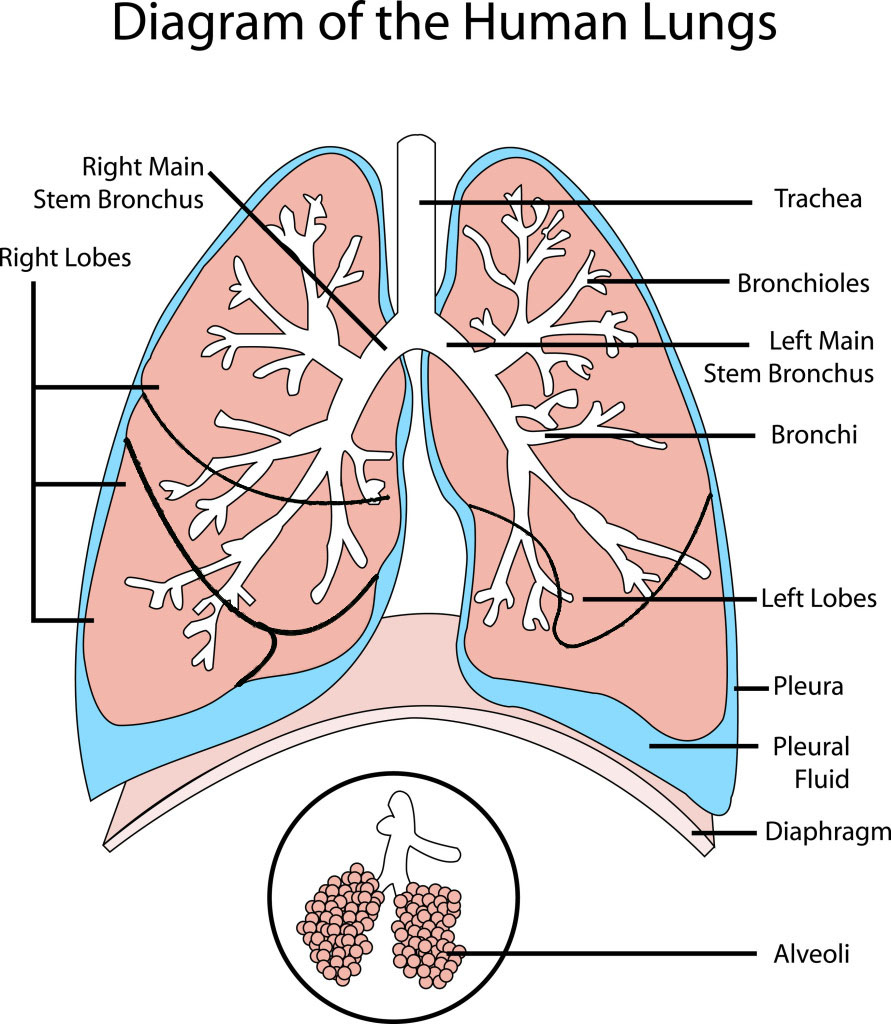
\includegraphics[height=2.7in]{Segmentation/Image/LobeAnatomicalStructure.jpg}
  \caption{Schematic diagram of anatomical lung structure, showing the major airways, lobes and major fissures. The lungs are subdivided into the right upper (RU), right middle (RM), right lower (RL), left upper (LU), and left lower (LL) lobe. The pleural cavity which surrounds the lung consists of a double membrane layer (visceral pleura and parietal pleura) separated by a thin layer of pleural fluid. The inner membrane (visceral pleural) folds inwards between the lobes, creating fissures. Reproduced from \citep{doel2015review}.}
  \label{fig:LobeAnatomicalStructure}
\end{figure*}

%%%%%%%%%%%%%%%%%%%%%
\subsection{High resolution computed tomography}
\gls{ct} imaging is a typical image modality used in diagnosis and management of IPF. It acquires multiple X-ray images at different orientations and reconstructs these images to obtain tomographic views in the region of interest \citep{zhang2011medical}. This kind of imaging modality is typically used in clinical applications and research regarding pulmonary structure-function relationships \citep{hoffman1997assessment}, including detection of both acute and chronic changes in the lung parenchyma. It is particularly relevant here because normal two-dimensional X-rays can not show subtle  defects. For evaluation of chronic interstitial processes (emphysema, fibrosis, and so forth), thin sections with high spatial frequency reconstructions are used \citep{coxson2007computed}, and scans are often performed both in inspiration and expiration. This special technique is called high resolution computed tomography (HRCT). With the help of \gls{hrct} scans, a series of high-resolution chest sections can be acquired with slice thickness as low as 0.5 mm \citep{naidich2005imaging}, which can provide high visibility of the lung boundaries and pulmonary fissures.  By making use of some advanced image processing technologies, a wide variety of features can be detected from these images such as density of the lung \citep{coxson2007computed}, volumes of the lung \citep{hu2001automatic}, the regions of lung disease distributions \citep{el2013computer, ley2008quantitative}, airway trees \citep{graham2010robust, zhu2010automatic, diaz2010airway} and blood vessels \citep{shikata2009segmentation}. CT images acquired at different stages in the breathing cycle can also be used to study lung mechanics and estimate regional lung ventilation \citep{hoffman2006state, yamamoto2011investigation}.

%%%%%%%%%%%%%%%%%%%%
\subsection{The importance of pulmonary lobar segmentation}
The extraction of pulmonary lobes from CT scans is of great importance for lung disease assessment and treatment planning. For clinical applications, the distribution and location of pulmonary disease are beneficial information for doctors to recognize pathogenesis, guide therapy and have further value in surgical planning. That is, because many pulmonary diseases are more prevalent in specific anatomic regions of the lung, often acting at a lobar level. For example, emphysema \citep{jeffery1998structural}, postprimary tuberculosis \citep{leung1999pulmonary} and silicosis \citep{rees2007silica} usually affect the upper lobes, while idiopathic pulmonary fibrosis is commonly present in the lower lobes \citep{lin2015combined}. However, there is currently a lack of quantitative and objective methods for the regional assessment of lung disease. Therefore, it is important to develop techniques that can identify the location, shape and volume of the lobes so that lung disease can be measured at a lobar level and the severity can be assessed accurately.

% Section 2
\subsection{Challenges of automatic pulmonary lobar segmentation from CT scans} \label{SegmentationChallenge}
The most commonly used method to segment lobes from CT is through manual assessment by an experienced pulmonary radiologist. However, the process of determining the lobar boundaries is extremely laborious and a time-consuming task, typically taking hours for one patient. This is because a 3D \gls{hrct} image may contain a large number of axial slices which makes the manual segmentation very time consuming. Therefore, doctors rarely use manual lobe segmentation in clinical diagnosis and treatment in practice, and most clinicians use subjective visual observation. For this reason, an automatic (no user interaction) or semi-automatic (minimal user interaction) lobe segmentation technique is urgently needed in clinical applications and this has attracted great interest from researchers all over the world \citep{van2013automated,pu2009computational,ukil2009anatomy}.

However, to find an effective and time-saving automatic lobe segmentation method is a challenging task because of anatomical variation and the possibility of incomplete fissures. Lobar structures vary significantly between subjects, and the anatomical variation in lobe structure is usually associated with age, sex and body type. Pathologies of diseased lungs usually deform the lobar shape abnormally and result in fuzzy appearance of fissures on \gls{ct} images, in particular when abnormalities are present near the fissures, which makes fissure segmentation challenging. Even in patients with healthy lung parenchyma, fissures are sometimes incomplete \citep{gulsun2006variability, doel2015review} (see Figure \ref{fig:FissureSegmentationChanllenges}).

\begin{figure*}[htbp]
  \centering 
  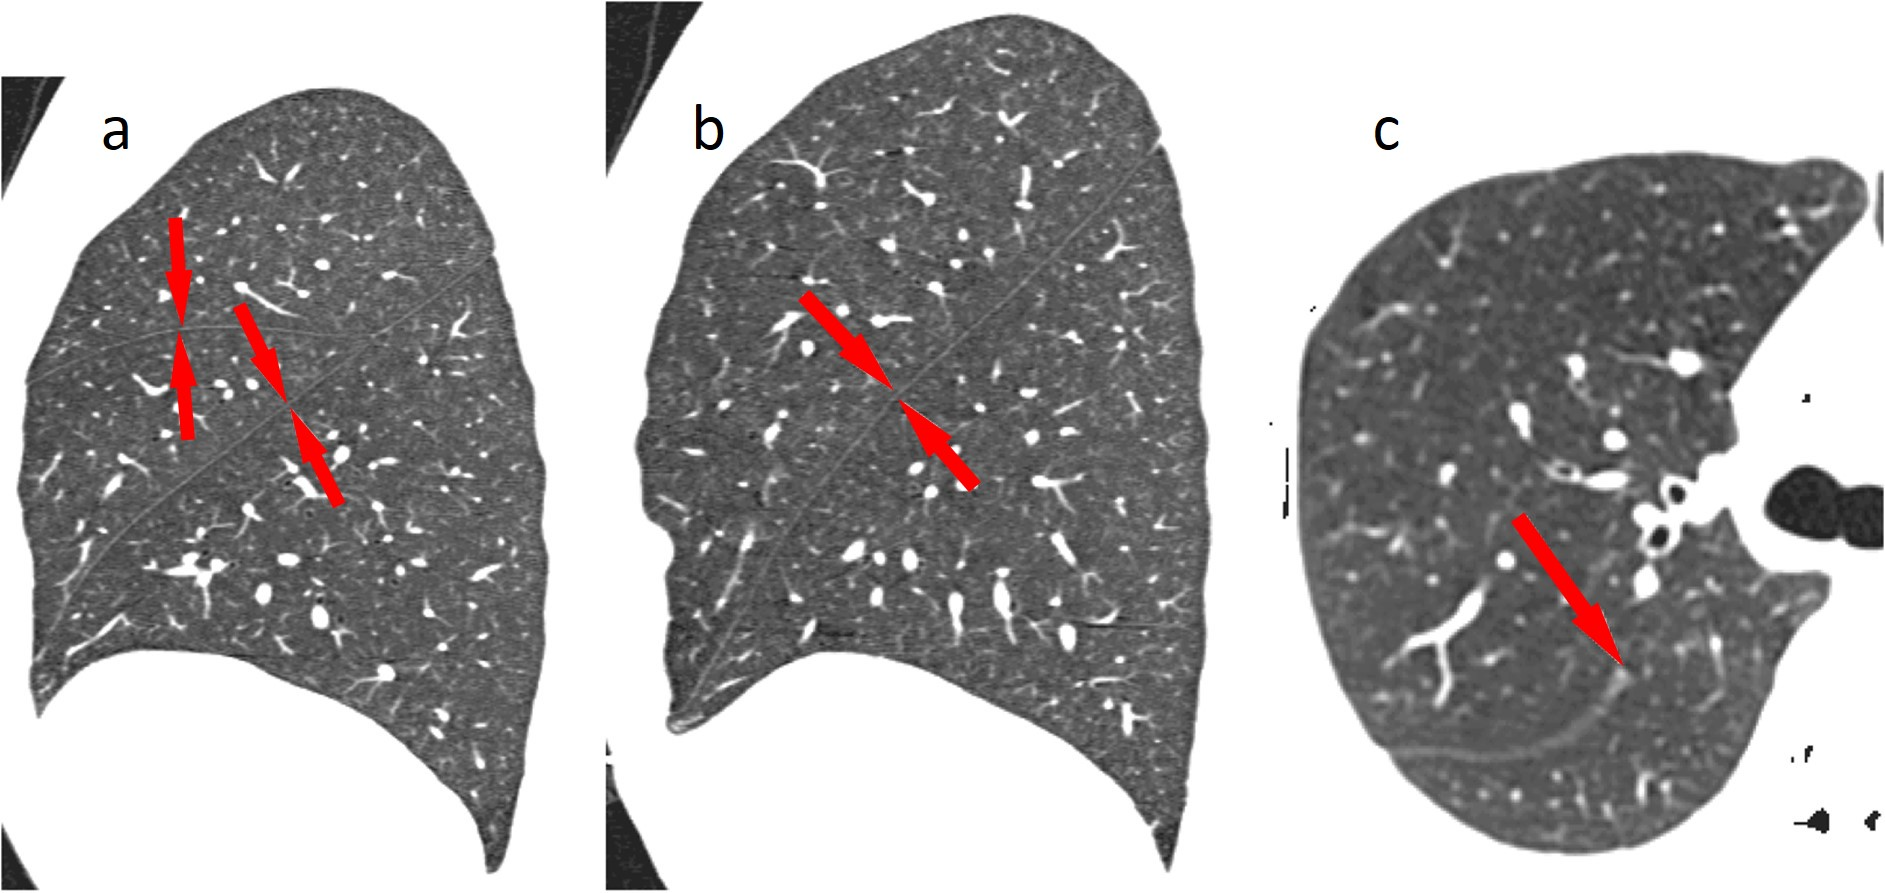
\includegraphics[height=1.75in]{Segmentation/Image/FissureSegmentationChanllenges.jpg}
  \caption{Slices of lung CT images illustrating the left and right fissures. Fissures are visible as white lines of high density tissue crossing the low density lung parenchyma. (a) Sagittal slice from the right lung showing the right oblique and horizontal fissures, the horizontal fissure is oriented horizontally. (b) Sagittal slice from the left lung showing the left oblique fissure. (c) Transverse slice from a different data set that show an incomplete right oblique fissure. Reproduced from \citep{ukil2009anatomy}.}
  \label{fig:FissureSegmentationChanllenges}
\end{figure*}

% Section 3
\section{Review of current published methods for pulmonary lobar segmentation} \label{SegmentationReview}
In a broad sense, existing lobe segmentation methods usually consist of two steps: the segmentation of lungs, and the detection of the three main pulmonary fissures \citep{van2013automated}. Currently, a number of lung segmentation methods are available and most produce reliable results for normal lung at end-inspiration \citep{hu2001automatic,ukil2005smoothing,sun20063d,pu2008adaptive,wang2009automated}. In contrast, most challenges of automated lobar segmentation lie in the fissure detection, and currently no method has yet been demonstrated to be robust and effective across a wide range of clinical imaging parameters and pathology experienced in clinical practice. Lung lobe segmentation is a complex multi-stage process that cannot be addressed by a simple algorithm \citep{van2013automated,pu2009computational,ukil2009anatomy}. However, to some extent, lung segmentation and fissure detection are two independent parts and can be improved separately. That is, it should be possible to change lung segmentation in one way or another without affecting the fissure detection result dramatically. In the following section, existing work is discussed to highlight the key challenges of lobe segmentation algorithms, focusing on these two parts of the process. Then, a new approach to lung and lobe segmentation is presented.

%%%%%%%%%%%%%%%%%%%%%%%%%%%%
\subsection{Lung segmentation}
Segmentation of lung is a prerequisite for the accomplishment of lobe segmentation, as it provides a boundary condition for subsequent fissure detection, allows estimation of lung volumes, and helps to detect and quantify abnormalities within the lungs. While not precisely defined, the lung region is usually considered to be the volume enclosed within the pleura, including the lung parenchyma, airways and vessels, but excluding those parts of the major airways and vessels which extend the pleural boundary. In this section, published methods for lung segmentation are briefly discussed. These methods are summarized in Table \ref{tab:LungSegmentationSummary}.

\newcolumntype{C}[1]{>{\centering\arraybackslash}p{#1}}
\begin{table}[htbp]
\centering
\caption{Summary of lung segmentation methods}
\label{tab:LungSegmentationSummary}
\begin{tabular}{|p{4.3cm}|p{6.3cm}|p{4.8cm}|}
\hline
\bf{Authors} & \bf{Algorithms} & \bf{Notes}\\ 
\hline
\cite{kalender1991semiautomatic,kemerink1998segmentation,leader2003automated} & 2D thresholding method &  1. May cause discontinuity between slices; 2. Time consuming\\
\hline
\cite{keller1981automatic,hedlund1982two,hoffman1983noninvasive,hoffman1985effectb} & Early-stage 3D thresholding method combined with manual interaction & Causes too many intra-operator errors\\
\hline
\cite{hu2001automatic} & 1. Automatically choose thresholding value; 2. Separate left and right lung 3. Morphological lung boundary smoothing & First group to apply fully automatic 3D thresholding method\\
\hline
\cite{ukil2005smoothing} & 1. Bounding box defined around mediastinum; 2. Extract left and right main stem bronchi; 3. 3D Morphological boundary closing & Automatic method using airway tree information\\
\hline
\cite{sun20063d} & 1. Anisotropic filtering; 2. Wavelet transform-based interpolation to construct 3D data; 3. Adaptive 3D region growing combined seed-locating to detect lung region; 4. Fuzzy logic algorithm and 3D morphological to fill hole & 3D method using signal-to-noise ratio\\ 
\hline
\cite{kitasaka2003lung} & 1. Affine transformation to fit a contour shape model to individual images; 2. Active contour model to refine initial segmentations in 3D & Solves the problem of lesions adjacent to the chest wall and mediastinum\\
\hline
\cite{pu2008adaptive} & 1. 3D initial thresholding processing; 2. Adaptive border marching & Minimizes oversegmentation of adjacent regions such as abdomen and mediatinum\\
\hline
\cite{pu2011shape} & 1. Principal curvature analysis to eliminate noise; 2. Radius basis function to smooth lung in 3D & Solves the problems of disease, noise or artifacts\\
\hline
\cite{prasad2008automatic} & 1. 3D thresholding algorithm; 2. Adapt lung curvature using rib curvature; 3. Morphologic operation & 1. Uses rib curvature information to define lung borders; 2. Solves the problem of error detection for lung pathologies\\
\hline
\cite{wang2009automated} & 1. 3D thresholding processing; 2. Texture analysis to identify abnormal regions; 3. 2D hole filling & Texture feature analysis to segment \gls{ild} lungs\\
\hline
\cite{sun2012automated} & 1. Active shape model to roughly find lung outlines; 2. Optimal surface finding to adapt final segmentations & 3D method using rib information\\
\hline
\end{tabular}
\end{table}

\subsubsection{Conventional lung segmentation methods}
In \gls{ct} scans from healthy subjects, the air-filled lung parenchyma usually has a lower attenuation level compared to surrounding high-density tissue at the pleura. For this reason, many conventional lung segmentation algorithms adopt a thresholding approach to search for a large connected region of the air-like values within the image. Threshold values are acquired from grey level histogram analysis and then an initial lung region is detected. A region growing method for the airways is usually applied subsequently to exclude the trachea and major airway branches. Some thresholding algorithms, especially older studies, were developed in 2D space, which means each axial section of \gls{ct} imaging needs to be analysed separately \citep{kalender1991semiautomatic,kemerink1998segmentation,leader2003automated,armato2004automated}. A 2-D method is a logical choice in the case of thick-slice \gls{ct} data, but it may cause discontinuity between slices. Therefore, as higher resolution isotropic data became available, improved 3D processing methods were developed to avoid slice inconsistencies and reduce time for segmentation \citep{hu2001automatic,ukil2005smoothing,sun20063d}.

Most early 3D thresholding-based lung segmentation methods \citep{keller1981automatic,hedlund1982two,hoffman1983noninvasive,hoffman1985effecta,hoffman1985effectb} required significant manual interaction. This interaction included manually selecting threshold values or seed points for region growing, and separating left and right lungs manually. This leads to a process that is consuming and is subject to intra-operator errors. \cite{hu2001automatic} was the first group to apply a threshold-based algorithm in a fully automatic lung segmentation method. In their study, the lung region was firstly extracted from the CT images by gray-level thresholding processing. Instead of a fixed threshold value, an optimal thresholding method was used to automatically choose a threshold value that reflects the grey-scale characteristics of a specific dataset. The left and right lungs were then separated by identifying the anterior and posterior junctions by dynamic programming. Finally, a sequence of morphological operations was used to smooth the irregular boundary along the mediastinum.

\cite{ukil2005smoothing} developed an improved automatic lung segmentation method to smooth lung boundaries in 3D using information from the segmented airway trees. A bounding box was first defined around the mediastinum for each lung using information from the segmented human airway trees, and all operations were then performed within the bounding box. After that, all generations of the airway distal branches were defined to the left and right main stem bronchi to be part of the respective lungs, and all the other segmented structures could be excluded. Finally, a fast morphological closing with an ellipsoidal kernel was performed to smooth the surface of the lung. This method solved the problem of irregular and inconsistent lung boundary of the regions near the mediastinum by using a common threshold algorithm. 

\cite{sun20063d} presented a 3D-based method for segmenting lungs with improved accuracy. An anisotropic filtering method was first applied on \gls{ct} slices to enhance the signal-to-noise ratio. A wavelet transform-based interpolation method was subsequently used to construct the 3D volumetric \gls{ct} slice data with volume rendering. After that, an adaptive 3D region-growing algorithm was developed to detect the lung region, combined with automatic seed-locating methods. Fuzzy logic algorithms and 3D morphological closing approaches were finally used to refine the lung volume and fill the holes in it. The method was effective and, in general, robust with an average accuracy rate of 88.5\%.  

\subsubsection{Specially designed lung segmentation methods for abnormal lungs}
Although conventional threshold-based methods are fast, robust and typically accurate for healthy subjects, they may fail to perform well for scans containing physiologic abnormalities, which often results in segmentation errors and requires manual editing of the results (see in Figure \ref{fig:AbnormalLungSegmentation}). Currently, specially designed lung segmentation methods mostly focus on a single lung disease and therefore can not get a good result across a large population \citep{kitasaka2003lung,sluimer2005toward,pu2008adaptive,pu2011shape,prasad2008automatic,korfiatis2008texture,wang2009automated,van2009automatic,sun2012automated}. 

\begin{figure*}[htbp]
  \centering 
  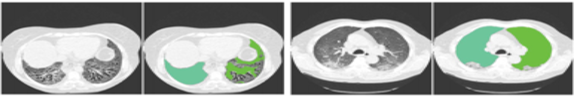
\includegraphics[height=1.5in]{Segmentation/Image/AbnormalLungSegmentation.png}
  \caption{Illustration of the performance of conventional 3D thresholding lung segmentation methods on pathological lungs. Lung borders are not recognized accurately because of the higher densities of the abnormalities compared to the normal tissues. Reproduced from \citep{van2013automated}.}
  \label{fig:AbnormalLungSegmentation}
\end{figure*}

To deal with the problem of lesions adjacent to the chest wall and mediastinum, \citep{kitasaka2003lung} developed a lung area extraction method using a shape model. A contour shape model using a B\'ezier surface was fitted to the contour surface of the individual input images with an affine transformation method. Then, an active contour model was utilized to refine the initial segmentation. The results showed that most lesions could be identified accurately using this method. However, as the lung apex and base were not included in the model, lesions adjacent to the lung apex or diaphragm could result in segmentation errors.

\cite{pu2008adaptive} presented a lung segmentation algorithm based on adaptive border marching (ABM) to include juxtapleural nodules in the lung region since these nodules may be excluded from the results calculated by a conventional threashold-based algorithm. The adaptive border marching algorithm could smooth the lung borders after an initial thresholding processing and minimize over-segmentation of adjacent regions such as the abdomen and mediastinum. The method was tested on 20 datasets and the results demonstrated that this method could re-include all juxtapleural nodules in the lung regions. An average over-segmentation ratio of this method was 0.43\% which was lower than the reference standard average segmentation determined by an expert. In order to deal with the problem of different types of lung disease, image noise or artefacts, and individual anatomical variety, \cite{pu2011shape} developed a shape analysis strategy termed ''break-and-repair''. A principal curvature analysis was applied to eliminate the problematic regions and then radial basis function (RBF) based implicit surface fitting was used to get a smooth lung surface. 

To overcome the error in detection of the lung boundaries for lung pathologies, \cite{prasad2008automatic} made use of rib curvature information to help with finding the lung borders. The method was based on a threshold-based algorithm followed by a morphologic operation. The core principle of the method was to adapt the threshold value to an individual subject by making the curvature of lung along the ribs be similar to the curvature of the ribs. These curvatures were both represented by polynomial interpolation even though there was minimal deviation from this representation. The results showed that the performance of the rib segmentation method was better than the same method without guidance from rib segmentation.

\cite{wang2009automated} proposed a texture analysis-based method to segment ILD lungs. The lung region including normal and mild ILD lung parenchyma was first segmented by a CT value thresholding technique and then texture-feature images derived from the co-occurrence matrix was used to identify abnormal lung regions with severe ILD from the initial results. 2D hole filling was applied to smooth the final lung segmentation. The overlap rate, volume agreement, mean absolute distance (MAD), and maximum absolute distance between the automatically segmented lungs and the reference lungs (delineated manually by a medical physicist) were employed to evaluate the performance of the segmentation method, and showed accurate lung segmentation results for abnormal CT scans with severe ILD.

On the basis of the previous studies, \citep{sun2012automated} developed a further approach for segmentation of lungs with high-density pathologies. The method had two main steps. In the first step, a robust active shape model (RASM) matching method was utilized to roughly find the outline of the lungs. To initialize the shape model of RASM, detected rib information was used. In the second step, an optimal surface finding approach was applied to further adapt the initial segmentation result to the lung. The method was evaluated on both normal and abnormal subjects and had a better performance compared to two commercially available lung segmentation approaches.
%%%%%%%%%%%%%%%%%%%%%%%%%%%%%%%%%%%
\subsection{Fissure detection}
The currently published fissure detection methods can be, for the most part, classified into two categories: anatomical knowledge based analysis methods and shape based analysis methods. Anatomical knowledge based methods usually depend on either local or global knowledge of the anatomy of lung structure based on two pulmonary anatomical features. The first feature is the fact that there should not be any large vessels in the vicinity of lobar fissures, so fissures should locate in the gaps between airway and vessel trees. Another feature is that the airway bronchi can be classified into five lobar branches using an edge detection method (Figure \ref{fig:AnatomicalBasedSegmentation}). Shape based analysis methods commonly make use of gray-level information and shape information to detect the fissures. Published fissure detection methods are summarized in Table \ref{tab:FissureDetectionSummary}.

\begin{figure}[htbp] 
\centering
\begin{subfigure}{.3\linewidth}% set image scale
  \sbox0{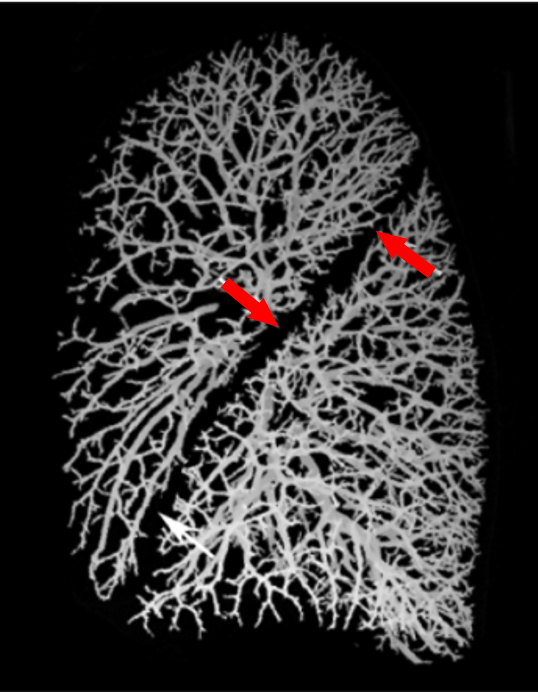
\includegraphics{Segmentation/Image/VolumetricVesselTree.png}}
  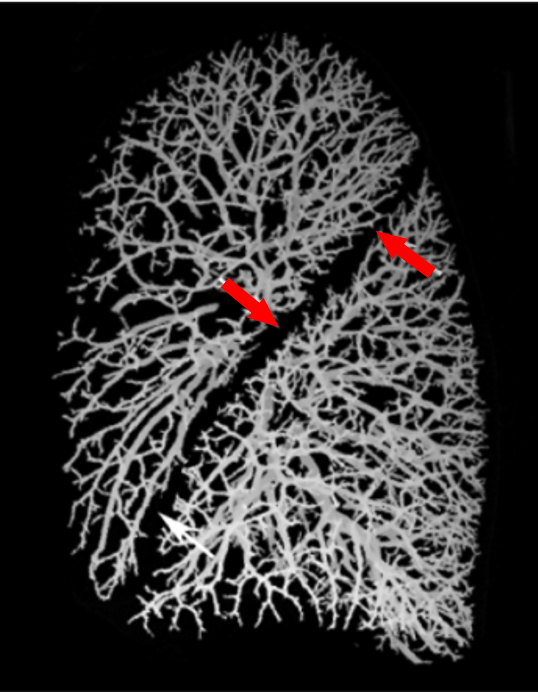
\includegraphics[width=\linewidth,trim={{.0\wd0} {.0\wd0} {.0\wd0} {.0\wd0}},clip]{Segmentation/Image/VolumetricVesselTree.png}
  \caption{}
  \label{fig:AnatomicalBasedSegmentation-a} 
\end{subfigure}
%\vspace{.3in} % control space between the upper context and figure
\hspace{.6in} % control space between two figures
\begin{subfigure}{.43\linewidth}% set image scale
  \sbox0{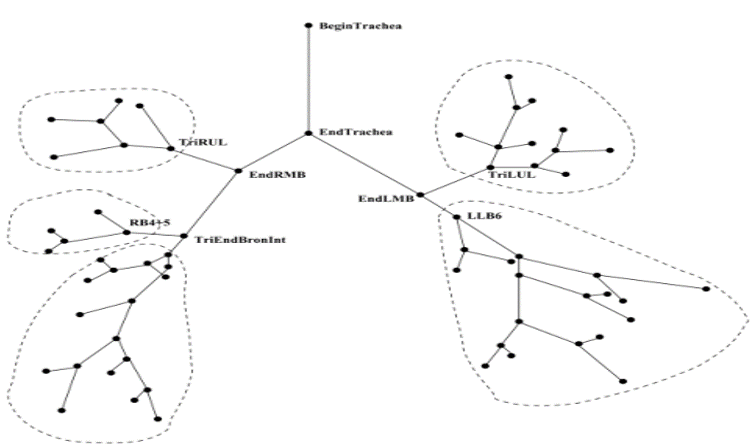
\includegraphics{Segmentation/Image/LabelledAirwayTree.png}}
  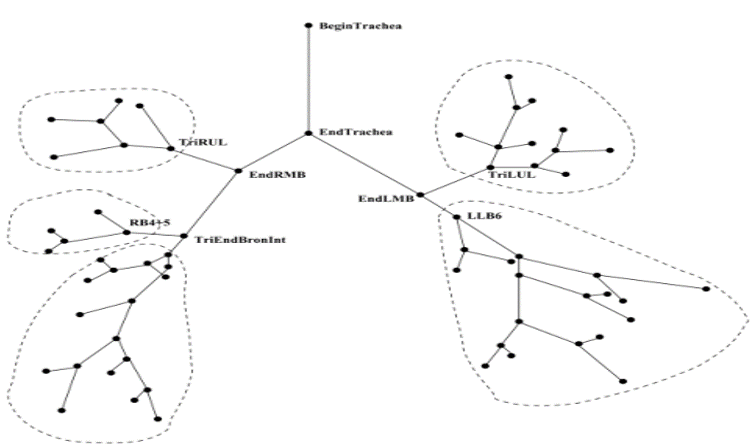
\includegraphics[width=\linewidth,trim={{.0\wd0} {.0\wd0} {.0\wd0} {.0\wd0}},clip]{Segmentation/Image/LabelledAirwayTree.png}
  \caption{}
  \label{fig:AnatomicalBasedSegmentation-b} 
\end{subfigure}
\caption{(a) Segmented volumes of the vascular tree. There are no large vessels in the vicinity of lobar fissures. (b) Anatomically labeled airway tree showing lobar subtrees. The airway tree can be classified corresponding to five lobes. Reproduced from \citep{ukil2009anatomy}.}
\label{fig:AnatomicalBasedSegmentation}
\end{figure}

\newcolumntype{C}[1]{>{\centering\arraybackslash}p{#1}}
\begin{table}[htbp]
\centering
\caption{Summary of fissure detection methods}
\label{tab:FissureDetectionSummary}
\begin{threeparttable}
\begin{tabular}{|p{4.3cm}|p{6.3cm}|p{4.8cm}|}
\hline
\bf{Authors} & \bf{Algorithms} & \bf{Notes}\\ 
\hline
\cite{kuhnigk2003lung,kuhnigk2005informatics} & Watershed transformation method to analyze anatomical structures to help with fissure detection &  First group to use lobar airways and vasulature into fissure detection\tnote{1}\\
\hline
\cite{ukil2009anatomy} & 1. Watershed transform guided cost image to define initial fissures; 2. Construct ROI; 3. Structure tensor analysis combined with optimal surface detection to find fissure surface; 4. Fast marching method to detect incomplete fissures & 1. Improved on Kuhnigsk's method; 2. Can detect incomplete fissures\tnote{1}\\
\hline
\cite{lassen2010automatic} & Watershed transformed anatomical structure based method & An extension of Kuhgigk's method\tnote{1}\\
\hline
\cite{zhou2004automatic,saita2006algorithm} & 1. Edge detection to class vessels and bronchi; 2. Hough transform to detect curve surface & Take advantage of linear appearance of fissures\tnote{1}\\
\hline
\cite{wang2004shape,wang2006pulmonary} & 1. Identify initial fissure ROI; 2. ''Ridge map'' based tranformation to enhance initial fissure; 3.  Shape-based curve growing to get the finial fissures. & 2D shape based method\tnote{2}\\
\hline
\cite{frangi1998multiscale} & Hessian matrix based analysis to extract local image structures & The first paper to apply Hessian matrix analysis on image segmentation in 3D\tnote{2}\\
\hline
\cite{wiemker2005unsupervised} & Combine first derivative and second derivative of image gray values to find fissures & An early paper using Hessian matrix on fissure detection\tnote{2}\\
\hline
\cite{ochs2007automated,van2008supervised} & Use pattern recognition approach and Hessian matrix and classification operation to detection fissure & An improved Hessian based method\tnote{2}\\
\hline
\cite{lassen2011interactive,lassen2013automatic} & 1. Use anatomical structures to acquire initial fissue; 2. Hessian matrix surrounding initial guessing areas; 3. Morphological operations to filter noise & Combine both anatomical information and gray-level information\tnote{1,2}\\
\hline
\cite{doel2012pulmonary} & 1. Use both anatomy knowledge and Hessian matrix to find fissure candidate points; 2. Multi-level B-spline curve to get the finial fissure surface. & Combine both anatomical information and gray-level information\tnote{1,2}\\
\hline
\cite{ross2010automatic,ross2013pulmonary} & 1. Particle system combined with Hessian matrix to get candidate fissure points; 2. Maximum a posterior method to remove noise points; 3. Thin plate spline to form finial fissure surface. & Effective for lung lobe segmentation in absence of complete anatomical structures on CT imaging\tnote{2}\\
\hline
\end{tabular}
\begin{tablenotes}
        \footnotesize
        \item[1] Anatomy knowledge based method.
        \item[2] Shape based analysis method.
\end{tablenotes}
\end{threeparttable}
\end{table}

\subsubsection{Anatomical knowledge based method}
Methods that aim to detect the lobar fissures usually start by finding an approximate location of the lobar borders based on prior anatomical knowledge of lung structures in order to narrow the search area for fissure detection \citep{kuhnigk2003lung,kuhnigk2005informatics,zhou2004automatic,saita2006algorithm,zhang2006atlas,ukil2009anatomy,pu2009computational,lassen2010automatic,doel2012pulmonary}. These methods are developed mainly based on two pulmonary anatomical features. A number of published papers use the segmentation results of airways and vessels to help localize fissures. Usually, the vascular segmentation provides more accurate estimation of lobar fissure locations than the airway trees, since more vessel generations can be detected from \gls{ct} scans. These vessels span the entire lung volume which can help to find complete gaps between lobes. However, airways also play an important part in initial estimation of fissures, since airways trees can be more reasonably divided into lobes based on branching structure, while the structure of vasculature branching is more complicated to extract from images and some connections are hard to separate accurately. Therefore, a lot of studies make use of both vessel and airway information to guide fissure detection \citep{ukil2009anatomy,lassen2010automatic,doel2012pulmonary}.

\cite{kuhnigk2003lung,kuhnigk2005informatics} was an early group to present a framework of taking both lobar airways and vasculature into account for automatic fissure detection. A watershed transformation method has been used to take an analysis of these anatomical structures and this method was widely used and improved by other researchers, but the results calculated by this simple algorithm were not accurate enough even for some clearly visible fissures. 

\cite{ukil2009anatomy} developed Khnigk's fissure detection method which used a distance transform to combine segmented vessels, lobar airways, and original chest CT scan as a cost image to guide initial fissure guessing. They found that the improved watershed transform algorithm could provide a close initial approximation to the lobar fissures. Subsequently, a refinement method was used to construct a region of interest (ROI) which encompasses the fissures. A 3D optimal surface detection algorithm combined with a 'ridgeness' measurement was then applied to enhance the ROI, and find the optimal surface within the ROI. Finally, incomplete fissures were smoothly extrapolated using a fast-marching method based segmentation of a projection of the optimal surface. This method is able to segment incomplete fissures, and so significantly improved on prior methods.

\cite{lassen2010automatic} also described a fissure detection method by building a cost image for the watershed transformed segmentation which is an extension of the framework of Kuhnigk. The interactive segmentation method was tested on 25 \gls{ct} scans comparing to a manual segmentation by a human observer and showed an average error distance of 1.57$ \pm $0.3mm. In addition, \cite{zhou2004automatic} and \cite{saita2006algorithm} took advantage of the linear appearance of fissures to class the vessels and bronchi into five lobe regions using an edge detection method and used a Hough transform based curved surface detection method. 

\subsubsection{Shape based analysis method}
Generally, lobar fissures can be regarded as bright planes crossing the pulmonary volume because of the higher density value of fissures compared to the surrounding tissues. Based on this information, quite a number of published methods use a local filtering algorithm to detect the voxels which lie on these planes, so that these detected voxel points can construct a continuous fissure surface. In 2D space, the fissure appears as a clear curve, therefore some early papers usually detected fissure points based on gray-level information in 2D space. For example, \cite{wang2004shape,wang2006pulmonary} presented a 2D fissure detection method based on shape information. In this paper, the fissure was initially denoted as a curve based on the prior knowledge of the fissure shape to identify the surrounding region of fissure, called ''fissure region'' for subsequent automatic segmentation. Next an image transformation called ''ridge map'' was proposed for enhancing the appearance of initial fissures. A shape-based curve-growing method modeled by a Bayesian network could then be applied to this ''map'' to segment the fissure.

In 3D space, the most commonly used method to detect these pulmonary fissure plane structures is taking an eigenvalue analysis of the Hessian matrix \citep{frangi1998multiscale,wiemker2005unsupervised,kitasaka2006recognition,ochs2007automated,van2008supervised,lassen2011interactive,lassen2013automatic,ross2010automatic,doel2012pulmonary}. \cite{frangi1998multiscale} was the first to present an eigenvalue analysis of the Hessian matrix to detect planar structures (fissures) and tube structures (vessels) on \gls{ct} images. The relationship between three eigenvalues of the Hessian matrix describes the local image structure and so can be used to determine a fissure probability. \cite{wiemker2005unsupervised} also used the Hessian matrix for fissure detection, proposing two 3D filter approaches in this paper. The first filter was based on the first derivatives of the image grey values and utilized the eigenvalues of the local structure tensor. The second filter was based on the second derivatives and utilized the eigenvalues of the local Hessian matrix. 

\cite{ochs2007automated} and \cite{van2008supervised} used a pattern recognition approach to detect pulmonary fissures combined with eigenvalue analysis of the Hessian matrix as feature and classification was also performed on these fissures. \cite{lassen2011interactive,lassen2013automatic} combined both anatomical based and shape based methods which successfully eliminated most false points (points identified as fissure but were not). The first anatomic-based method defined a region of interest, and then the Hessian matrix analysis was used only in this region of interest. The region of interest provides an initial guess for fissure locations. Subsequently, morphological operations such as direction-based connected component analysis were used to further reduce non-fissure points that are incorrectly identified as fissures. \cite{doel2012pulmonary} also made use of both an anatomical knowledge based method and the Hessian matrix to find fissure candidate points and constructed a multi-level B-spline smooth curve through the fissure points and extrapolated this curve to the lung borders to get complete fissure surfaces.

\cite{ross2010automatic, ross2013pulmonary} proposed a particle system that sampled the image domain combined with the Hessian matrix to get a set of candidate fissure locations. A maximum a posteriori (MAP) estimation was then used to eliminate false candidate points, and a post-processing operation was applied to remove remaining noise. A thin plate spline (TPS) interpolating surface fitting method was lastly performed to form the final fissure surfaces. This method is effective for lung lobe segmentation in the absence of complete anatomical structures on CT imaging.

%%%%%%%%%%%%%%%%%%%%%%%%%%%%%%%%%%%%%%%%%%%%%%5
% Section 4
\section{Methods: automatic statistical shape model based lobar segmentation method} \label{SegmentationMethod}
Here, an \gls{ssm} guided method is presented to segment pulmonary lobes from \gls{ct} images. A three-step approach is followed for the lobe segmentation (shown in Figure \ref{fig:WholeWorkflow}): in the first step, a threshold-based lung segmentation method defines the lung boundary; in the second step, an \gls{ssm} is deformed to provide a ''search region'' for fissure locations; in the third step, fissures are located using a Hessian matrix protocol combined with connected component filters and a surface fitting algorithm. The new procedure does not depend on prior segmentation of anatomical structures (airway lobar classification) other than lung shape. A user-interactive interface was also developed for the user to control and visualize the whole segmentation process and to allow some manual correction on the segmented results, if required.
\newpage

\begin{figure}[H]
  \centering 
  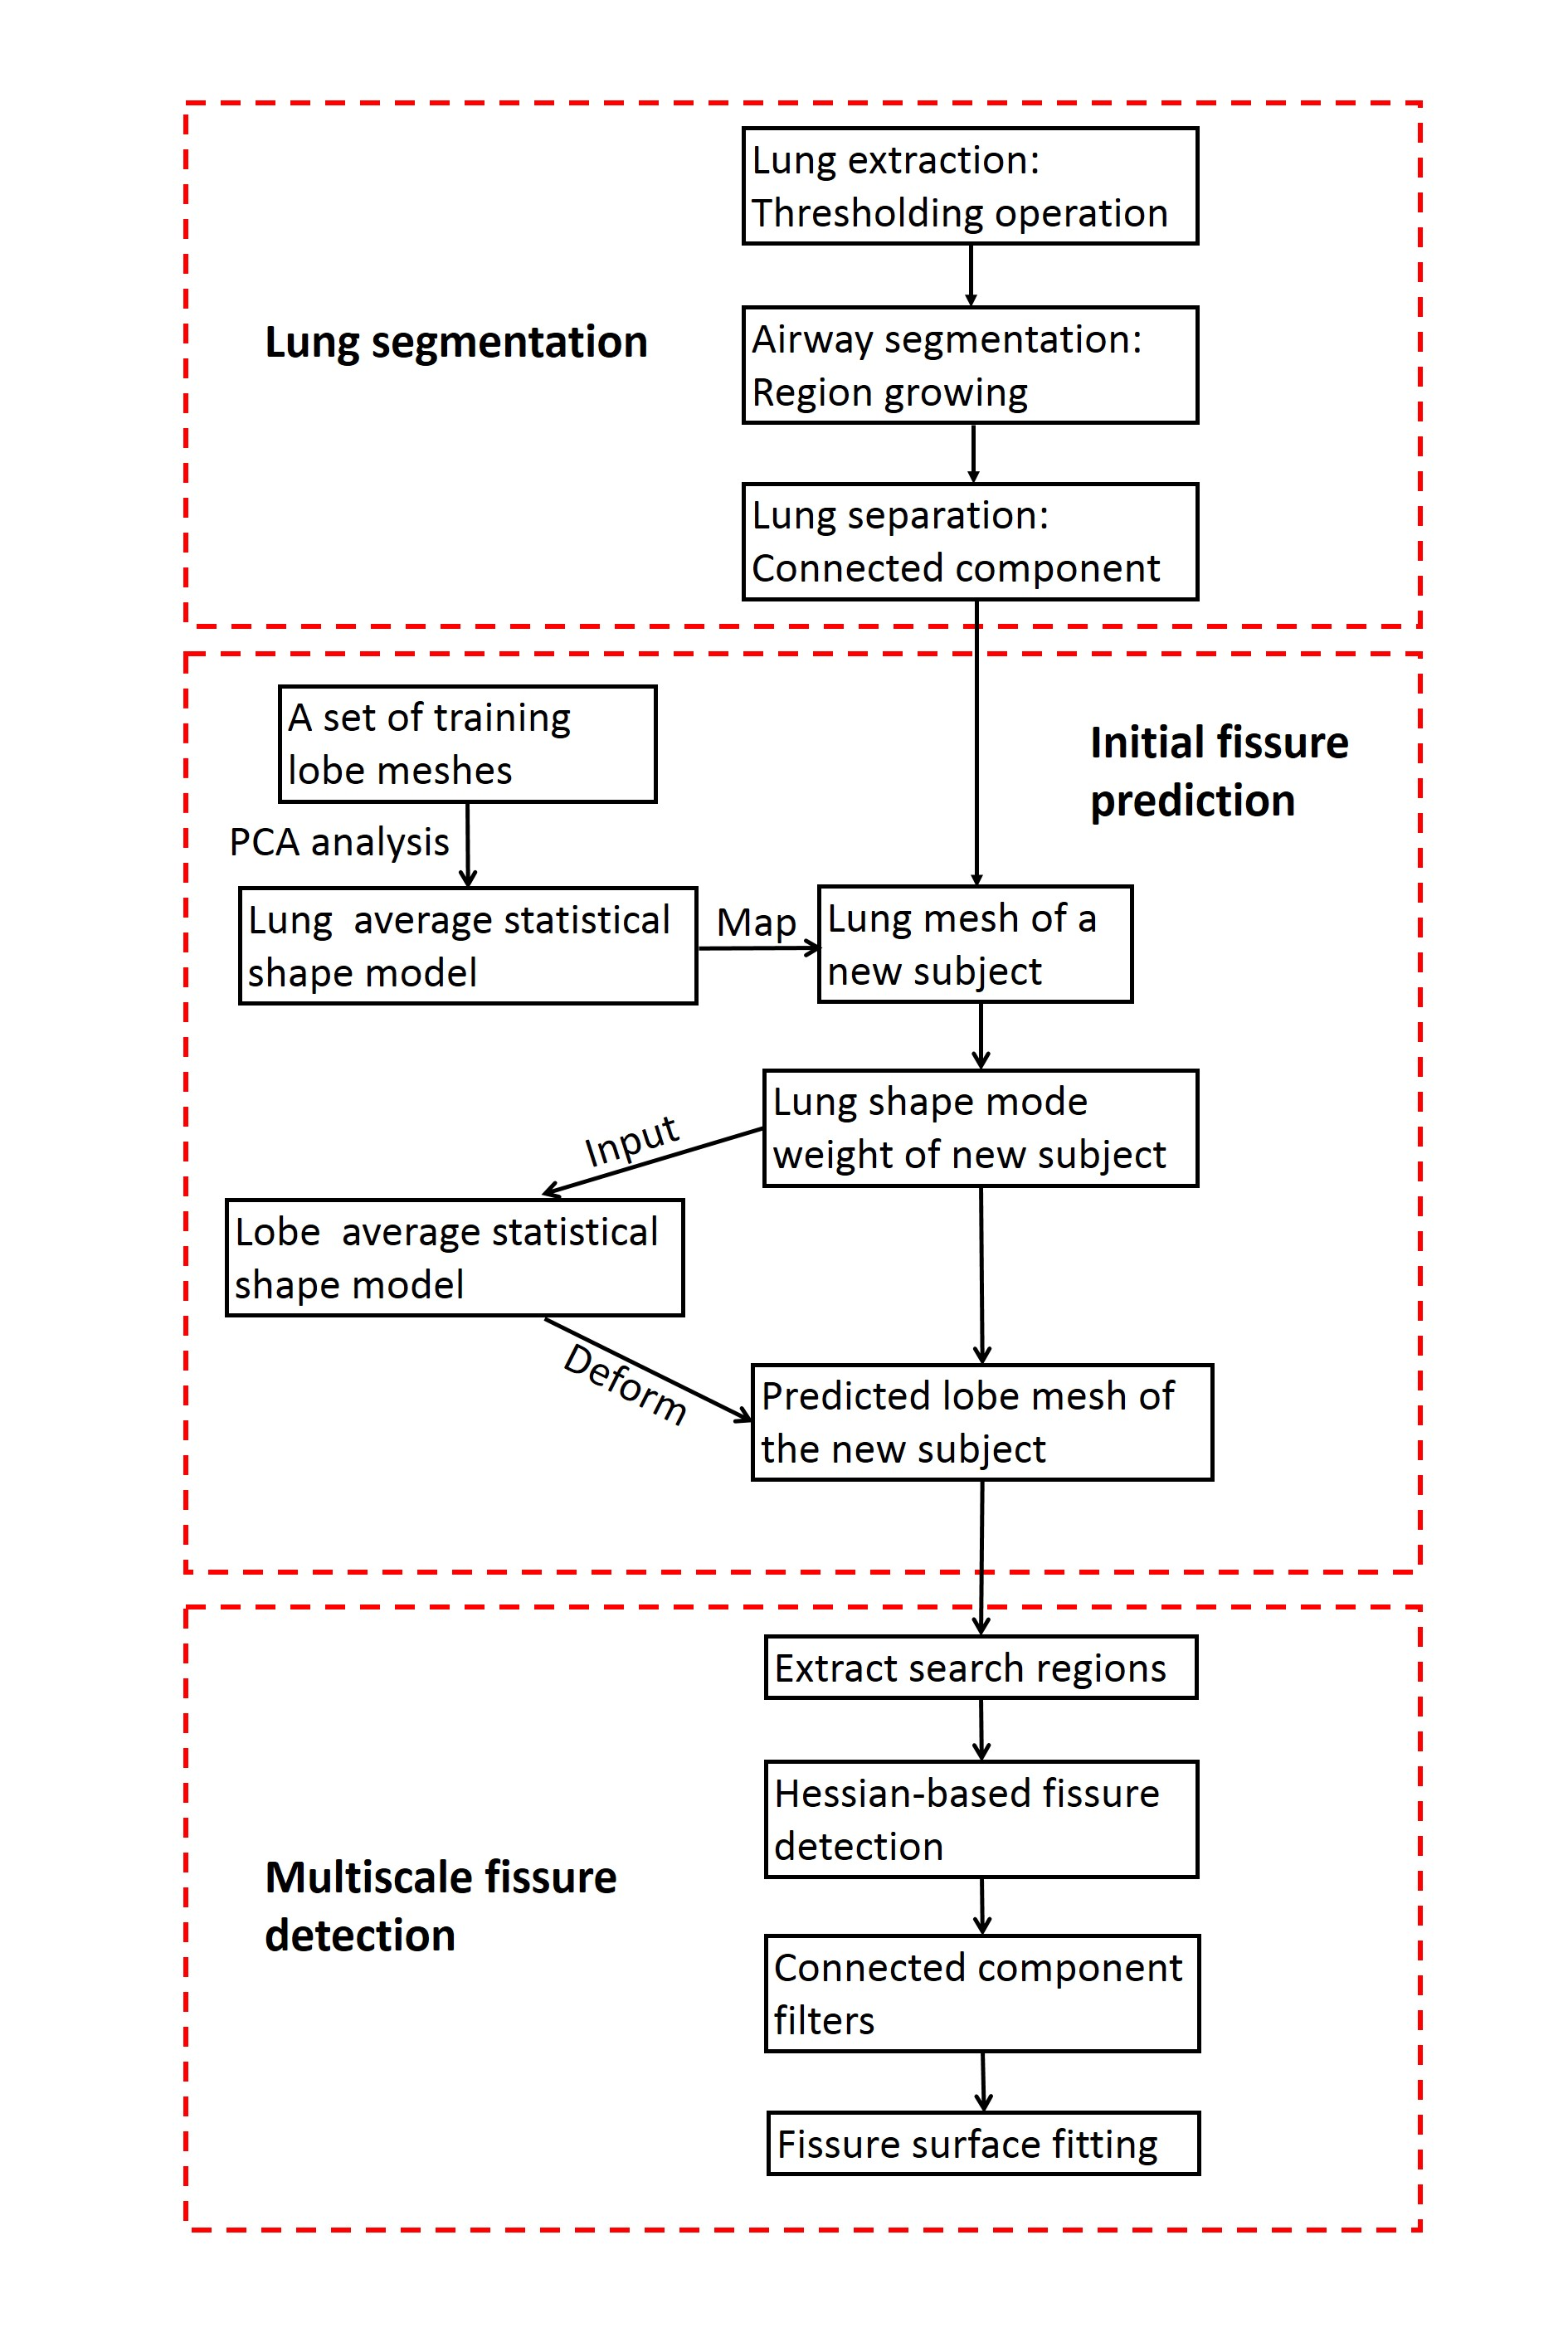
\includegraphics[height=7.8in]{Segmentation/Image/WholeWorkflow.jpg}
  \caption{Flow diagram of the lobar segmentation process.}
  \label{fig:WholeWorkflow}
\end{figure}

%%%%%%%%%%%%%%%%%%%%%%%%%%%%%%%
\subsection{Lung segmentation} \label{subsection:LungSegmentation}
A good lung segmentation is a prerequisite for lobe segmentation, since all the other segmentations need to be performed inside the two lung regions. Here, a common thresholding method was used to segment the lungs \citep{ukil2005smoothing}. The procedure consists of the following steps: 1) uses a thresholding operation (-775 Hounsfield Units) and connected component identification to find the initial lung regions and trachea location, 2) by using the most apical point of the trachea as a starting point, a region growing technique is applied to detect the airway trees, and 3) left and right lungs are separated as the two largest connected components remaining after removing the trachea and main left and right bronchi. Figure \ref{fig:LungSegmentation} shows a typical lung segmentation result.

\begin{figure}[htbp] 
\centering
\begin{subfigure}{.4\linewidth}% set image scale
  \sbox0{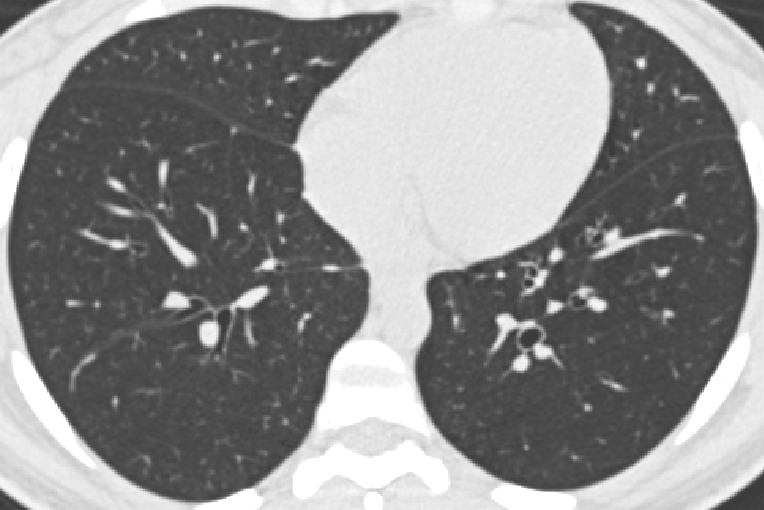
\includegraphics{Segmentation/Image/LungSegmentationBefore.png}}
  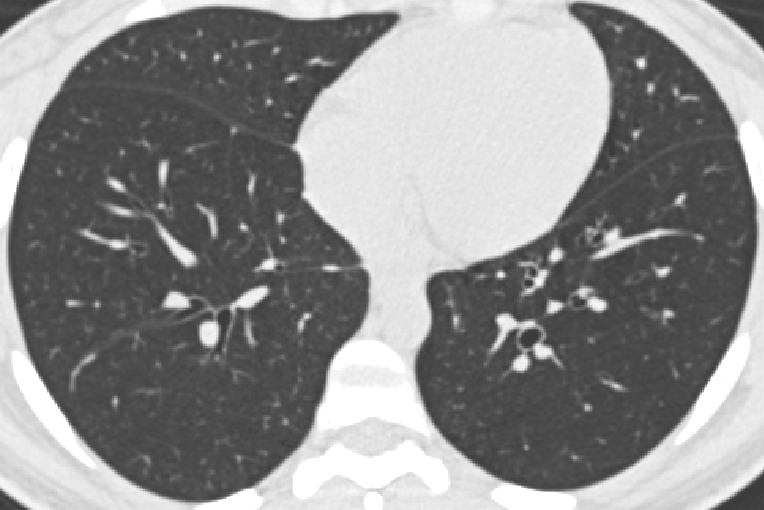
\includegraphics[width=\linewidth,trim={{.0\wd0} {.0\wd0} {.0\wd0} {.0\wd0}},clip]{Segmentation/Image/LungSegmentationBefore.png}
  \caption{}
  \label{fig:LungSegmentation-a} 
\end{subfigure}
\begin{subfigure}{.4\linewidth}% set image scale
  \sbox0{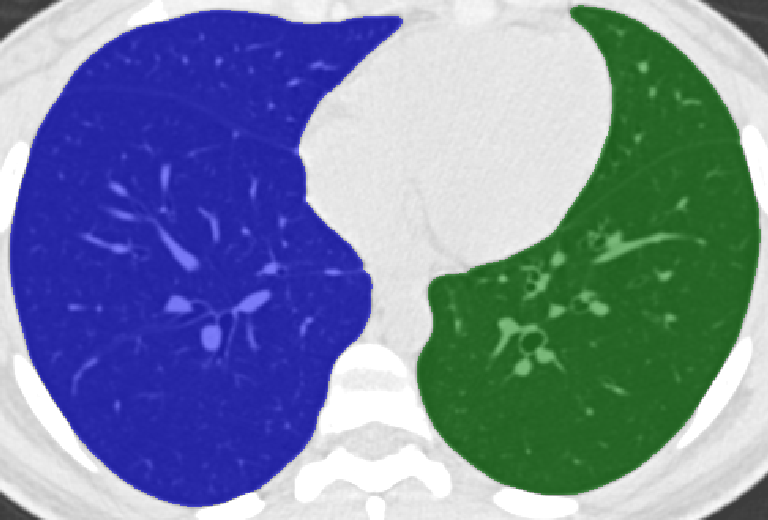
\includegraphics{Segmentation/Image/LungSegmentationAfter.png}}
  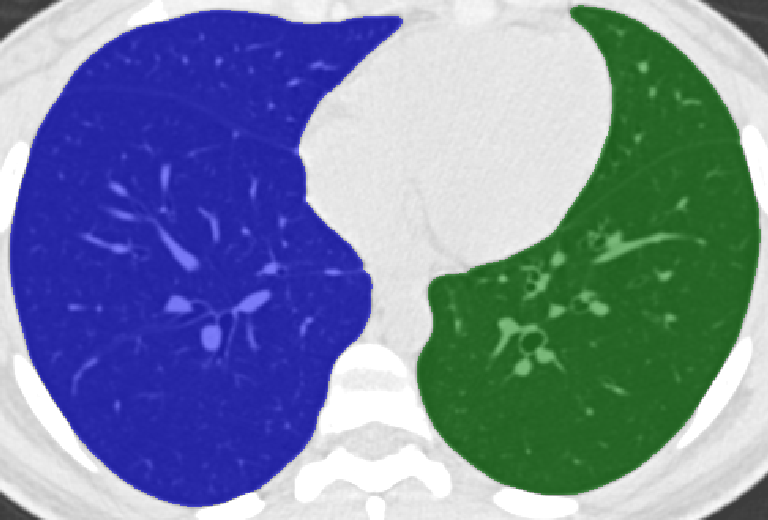
\includegraphics[width=\linewidth,trim={{.0\wd0} {.0\wd0} {.0\wd0} {.0\wd0}},clip]{Segmentation/Image/LungSegmentationAfter.png}
  \caption{}
  \label{fig:LungSegmentation-b} 
\end{subfigure}
\caption{Lung segmentation result using the common thresholding method. (a) Raw CT image. (b) Segmented lungs.}
\label{fig:LungSegmentation}
\end{figure}

%%%%%%%%%%%%%%%%%%%%%%%%%%%%%%%%%
\subsection{Statistical finite element models of lung and fissure shape} \label{ShapeModelGeneration}
For human organs, there is a significant difference in shape and anatomy between different groups of people, such as young and old, male and female, healthy and diseased \citep{krumpe1985aging, crapo1993aging}. This difference is caused by different functional signals and behaviours, leading to organ shape variation across populations. Shape analysis provides a way to understand the underlying mechanisms of those variations in anatomical and physiological processes. The importance of statistical shape analysis in many kinds of biological studies has been well established \citep{dryden1998statistical,stegmann2002brief,styner2003statistical,heimann2009statistical}, because of its potential to capture morphological variation within and between healthy and pathological structures.

Computational model-based approaches to solve problems in image segmentation have become increasingly popular in the last two decades \citep{taylor1995medical,kelemen1999elastic,tsai2003shape,okada2008automated}. In these approaches, each new image set was matched to its expected shape of organ for that individual as a guide for segmentation. This potentially reduces the impact of image artefacts and other perturbations associated with traditional low-level algorithms \citep{ecabert2008automatic,zhang2013development}. To account for individual variations in lung shape and location of fissures (including how they vary with lung inflation), one can analyse a series of training shapes using statistical techniques, leading to a statistical shape model. Using this statistical definition of a cohort of individuals, one can begin to predict an individual's organ shape based on characteristics of that individual to help guide segmentation procedures.

%%%%%%%%%%%%%%%%%%%%%%%%%%%%%%%%%
\subsubsection{Finite element lobar shape modeling} 

To guide a statistical shape model based segmentation, the first step is to generate a statistical lobar shape mesh using a set of training data. Here, we employ a \gls{sfeal} based on an active shape model (ASM) \citep{cootes1995active}. To do this, a training set of segmented lung and fissure surface locations was used to describe a cohort of adults with radiologically normal lungs. This approach employs a finite element shape mesh to specify pulmonary lobar shape which provides an efficient parameterized representation of lobar boundaries and makes shape constraints available during image analysis. The training set consisted of data from 50 subjects. 35 subjects were selected from a study of healthy subjects aged 50 to 100 years, the \gls{aging} study and a further 15 subjects were selected from a separate study of younger healthy subjects, the \gls{hla}. All the \gls{aging} and \gls{hla} subjects are healthy non-smoking subjects including both males and females. In the \gls{aging} group, \gls{hrct} imaging was acquired at Auckland City Hospital using a Phillips Brilliance 16 scanner, with between 400-700 slices per volumetric image. The study was approved by the Northern A Health and \gls{hdec}, Ministry of Health on 29 April 2013 through the \gls{hdec}-Full Review Pathway - ethics reference 13/NT/41. The \gls{hrct} images from \gls{hla} cohort were obtained at the \gls{iclic} using a Siemens Sensation 64 MDCT scanner, with between 500-700 slices per volumetric image. The study was approved by the University of Iowa Institutional Review Board. A summarized population demographics of the subjects used for statistical shape model construction is listed in Table \ref{tab:SSMSubjects}

\begin{table}[htbp]
\centering
\caption{Summarized demographics for the AGING and HLA datasets.}
\label{tab:SSMSubjects}
\begin{tabular}{l c c}
\hline
  & AGING (N=35) & HLA (N=15)\\ 
\hline
Age (years) & 72.3$ \pm $11.41 &  22$ \pm $1.9\\
Sex(M/F) & 18/17 & 5/10\\
Height(m) & 1.66$ \pm $0.14 &	1.7$ \pm $0.1\\
Weight(kg) & 70.6$ \pm $11.1 &	67.6$ \pm $12.2\\
BMI(kg/$\mathrm{m^{2}}$) & 25.6$ \pm $3.0 &	23.3$ \pm $2.2\\
\hline
Ethnicity\\
- Caucasian & 25 &	14\\
- M$\mathrm{\bar{a}}$ori(AGING only) & 1 &	N/A\\
- Asian & 2 &	-\\
- African-American & - &	1\\
 - Unknown & 7 &	-\\
\hline
\end{tabular}
\end{table}

To define the lung shape, volumetric \gls{ct} images were segmented using the method described in Section \ref{subsection:LungSegmentation}. The segmented lung surface was then digitized into a set of data points as a 3D-space representation of lung shape (Figure \ref{fig:LobeShapeGenereation-a}). Fissure surface segmentation was performed manually using the open-source visualization software CMGUI (https://www.cmiss.org/cmgui) by an expert user, to provide a gold-standard definition of the fissure location for each subject in the training set (Figure \ref{fig:LobeShapeGenereation-b}, \ref{fig:LobeShapeGenereation-c}). A high order (bi-cubic Hermite) finite element template mesh with the same mesh connectivity for each subject was geometry fitted to the lung and fissure surface data for each subject. The current lung lobe mesh consists of two separate meshes which represent the left and right lung enclosing the lung parenchymal tissue volume. 

An initial template mesh was created by selecting some data points to be nodes, and then creating two-dimensional surface elements by joining these node points appropriately. The template mesh for the left lung mesh has 35 nodes and 44 elements which described the left lung surface and left oblique fissure, while the right lung mesh has 50 nodes and 62 elements which defined right lung surface, right oblique fissure and right surface fissure. For fitting to lung and lobe shape data, the template mesh was modelled using bi-cubic Hermite basis functions with C1 continuity. This bi-cubic Hermite mesh has the same mesh connectivity as the template mesh, but it also contains nodal derivative information. Each node has 12 \gls{dof}s which store the global coordinates (x, y and z) and first and second nodal derivatives (\pd{n}{\xi_1}, \pd{n}{\xi_2}, and \pd[2]{n}{\xi_1 \xi_2}), where n is x, y and z, and $\xi$ is the local element coordinate. In this lung lobe model they are defined such that $\xi_1$ is in the anterior-posterior direction while $\xi_2$ is in the cranio-caudal direction. $\xi_1$ and $\xi_2$ have values that range from 0 to 1. Each node of the fitted mesh is either an anatomical landmark (the left/right lung apex, the base vertex, the shape corner and the centre point of the middle line of fissure) or a pseudo-landmark (e.g. a specific proportion of the arc-length between two anatomical landmarks). These landmarks allow the coordinate of the control points to be defined in consistent positions registered to the geometry of the lung. A least squares fit of the mesh to the lung and fissure surface data was conducted using CMISS ({https://www.cmiss.org), which is a finite element modelling environment. Specifically, the sum of the distances between each data point and its projection on to the nearest element was minimized during the fitting process. This distance is a function of the element location and shape parameters. In this procedure, the nodal parameters are interpolated to find the projected points. The global coordinates of the projected points are a function of local element coordinates, $\xi_1$ and $\xi_2$, and nodal parameters. Some manual operations were involved to adjust the mesh nodal positions and derivatives to the data cloud, which can help to improve the speed and accuracy of fitting. The average \gls{rms} error of this fitting method was 4.79 mm for the 50 training subjects (Figure \ref{fig:LobeShapeGenereation-d}). More details on the fitting procedure can be found in  \citep{bradley1997geometric,tawhai2003developing, fernandez2004anatomically}.  


\begin{figure}[htbp] 
\centering
\begin{subfigure}{.43\linewidth}% set image scale
  \sbox0{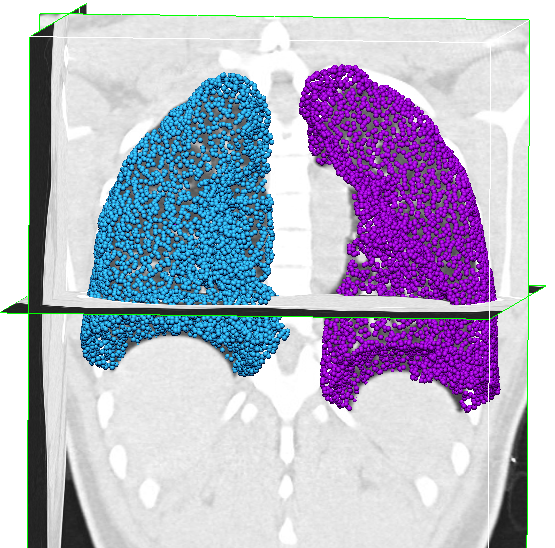
\includegraphics{Segmentation/Image/LungDigitising.png}} 
  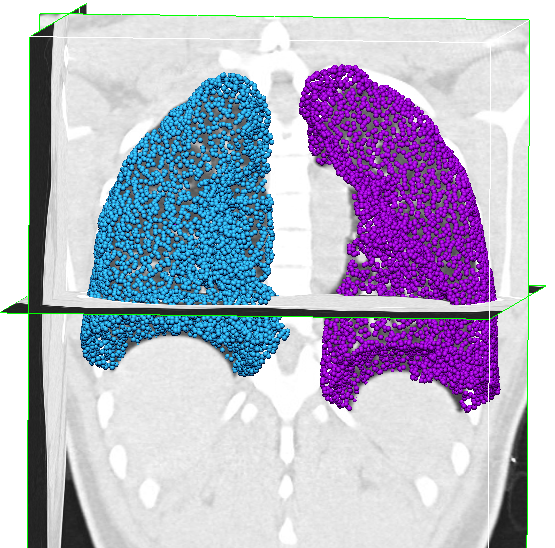
\includegraphics[width=\linewidth,trim={{.0\wd0} {.0\wd0} {.0\wd0} {.0\wd0}},clip]{Segmentation/Image/LungDigitising.png} %trim={<left> <lower> <right> <upper>}, set the cut scale
  \caption{}
  \label{fig:LobeShapeGenereation-a} 
\end{subfigure} 
%\vspace{.3in} % control space between the upper context and figure
\hspace{.3in} % control space between two figures
\begin{subfigure}{.325\linewidth}% set image scale
  \sbox0{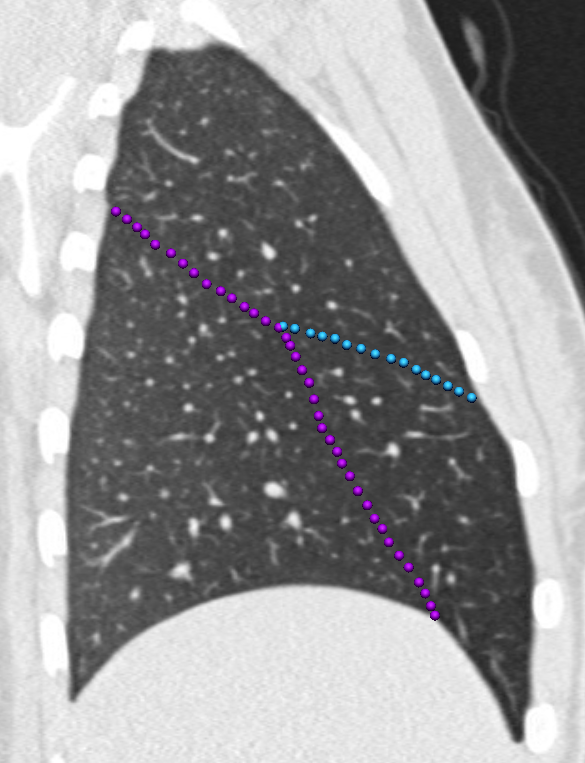
\includegraphics{Segmentation/Image/FissureDigitising1.png}}
  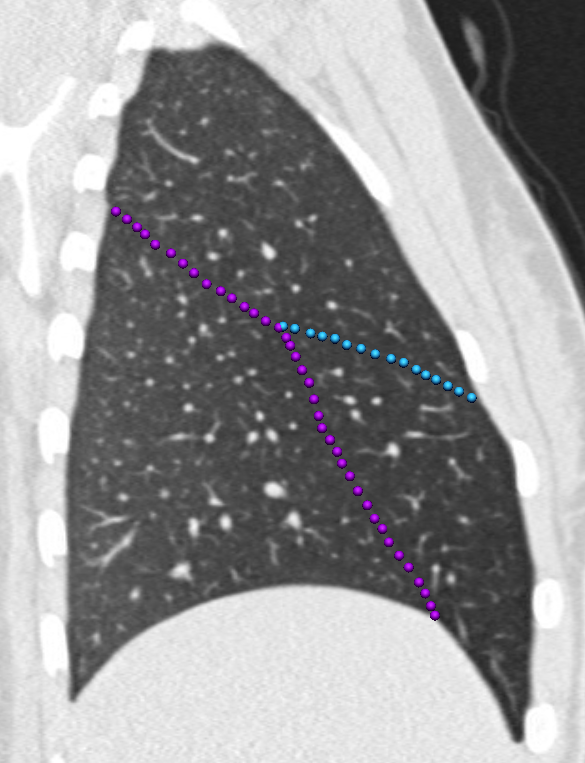
\includegraphics[width=\linewidth,trim={{.0\wd0} {.0\wd0} {.0\wd0} {.0\wd0}},clip]{Segmentation/Image/FissureDigitising1.png}
  \caption{}
  \label{fig:LobeShapeGenereation-b} 
\end{subfigure}
\begin{subfigure}{.48\linewidth}% set image scale
  \sbox0{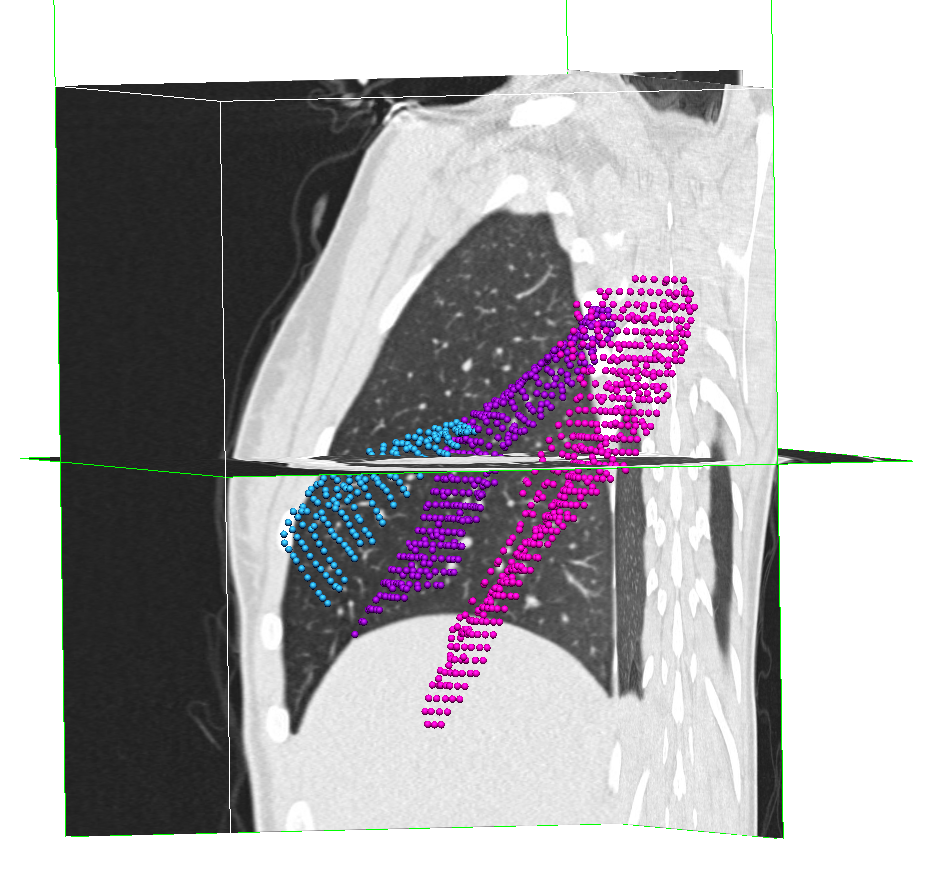
\includegraphics{Segmentation/Image/LobeDigitising.png}}
  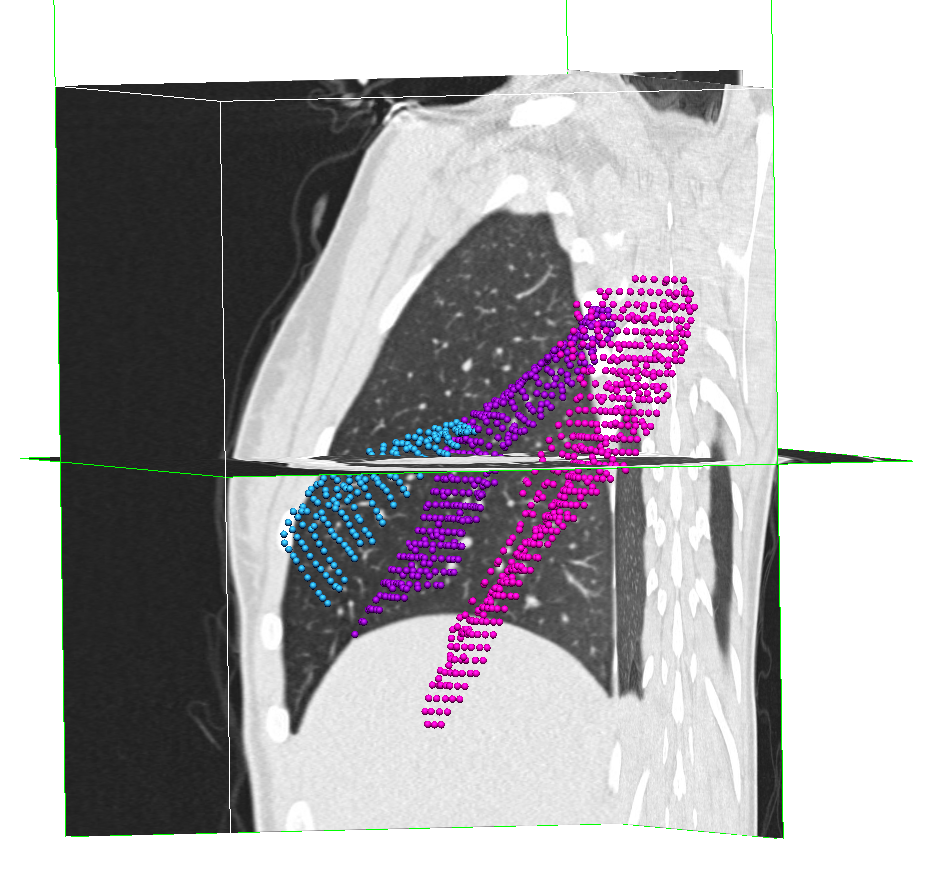
\includegraphics[width=\linewidth,trim={{.0\wd0} {.0\wd0} {.0\wd0} {.0\wd0}},clip]{Segmentation/Image/LobeDigitising.png}
  \caption{}
  \label{fig:LobeShapeGenereation-c} 
\end{subfigure}
%\vspace{.3in} % control space between the upper context and figure
\hspace{.3in} % control space between two figures
\begin{subfigure}{.32\linewidth}% set image scale
  \sbox0{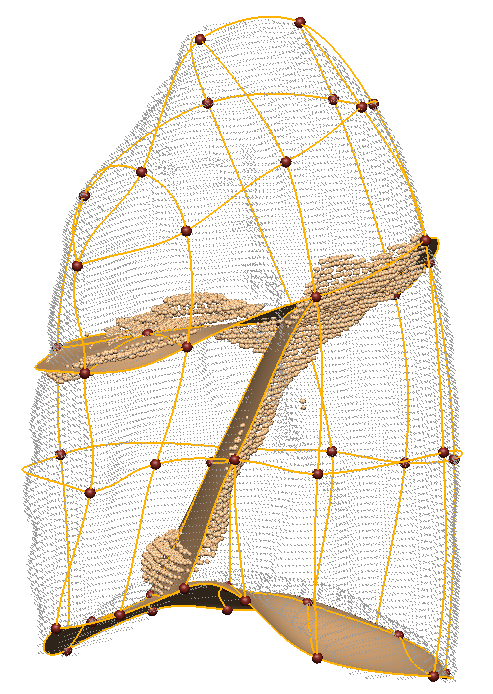
\includegraphics{Segmentation/Image/LobeFitting2.png}}
  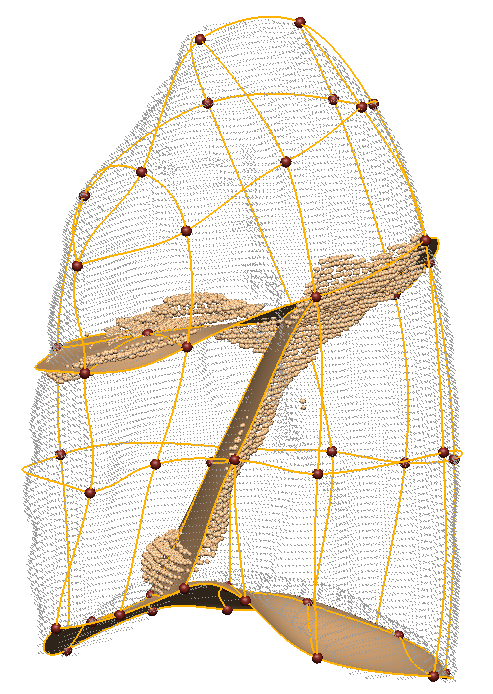
\includegraphics[width=\linewidth,trim={{.0\wd0} {.0\wd0} {.0\wd0} {.0\wd0}},clip]{Segmentation/Image/LobeFitting2.png}
  \caption{}
  \label{fig:LobeShapeGenereation-d} 
\end{subfigure}
\caption{Finite element modeling of lung lobe shape. (a) Lung surface data extracted from segmented lung masks (purple points for left lung, blue points for right lung). (b) Manual digitized fissure points in 2D sagittal image of right lung (purple points for right oblique fissure, blue points for right horizontal fissure). (c) Manual digitized fissure points shown in 3D (pink points for left oblique fissure, purple points for right oblique fissure, blue points for right horizontal fissure). (d) Lobe shape fitting with lung surface data and digitized fissure data of right lung.}
\label{fig:LobeShapeGenereation}
\end{figure}

%%%%%%%%%%%%%%%%%%%%%%%%%%%%%%%%%
\subsubsection{PCA-based statistical shape model construction} \label{SSMConstruction}

A prerequisite of the construction of an SSM is object alignment to remove the orientation and scaling differences between shapes. Here a \gls{gpa} was selected as a registration method \citep{dryden1998statistical,rohlf1999shape}. The GPA algorithm finds the optimal rotation matrix and translation vector which minimizes the overall distance between two sets of points with respect to the Euclidean norm. In this study, a reference lung model sample was randomly chosen from the training set. Then all the other training models were aligned to this reference model. In this process, the volumes of all subjects were normalized to 1 L and any residual rotation and translation were removed. The generalized procrustes alignment can be represented as an affine transformation in mathematical terms

\begin{equation}
 \label{eq:PCAConstruction1}
 \bar{S} = \alpha RS + T,
\end{equation}

\noindent where $\bar{S}$ represents the aligned shape vector to the reference shape from the subject shape vector S, R is the rotation matrix and T is the translation vector. Figure \ref{fig:PCAMeshTraining-a} shows the procrustes aligned meshes of all the 50 subjects. For each subject, the aligned lung shape can also be represented as 

\begin{equation}
 \label{eq:PCAConstruction2}
 \bar{S} = [\mathbf{\bar{x}}_1 \; \mathbf{\bar{x}}_2 \; \mathbf{\bar{x}}_3 \; \cdots \; \mathbf{\bar{x}}_{p-1}; \mathbf{\bar{x}}_p],
\end{equation}

\noindent where $\bar{x}$ are the nodal parameters which contain coordinates and derivatives (12 \gls{dof}s), and p represents the number of nodes for both left and right lung (p = 225 in this study). The data vector $\bar{S}$ of each lung was then assembled as the concatenation of all lungs, termed $\bar{S}_{whole}$. $\bar{S}_{whole}$ is an n$\times$N matrix, where n is the number of nodal parameters for each lung (n = 12 $\times$ 225 = 2700 in this study), and N is the number of training subjects (N = 50). Thus, $\bar{S}_{whole}$ can be regarded as a cloud of N points in the constructed n-N space. This matrix was decomposed into modes of variation using \gls{pca}. \gls{pca} is a commonly used technique in statistical feature space to reduce the dimension of the dataset. It uses an orthogonal transformation to convert a number of (possibly) correlated variables into a set of values of linearly uncorrelated variables called principal components. The number of distinct principal components is equal to the smaller of the number of original variables or the number of observations minus one. The resulting vectors are an uncorrelated orthogonal basis set. 

In order to perform PCA, each shape parameter was centred by subtracting the mean value $\mathbf{\bar{x}}$. Then the covariance matrix was built based on the mean-centred matrix S by $C = SS^T$. After the PCA technique was performed on the covariance matrix C, we obtain a set of eigenvectors $\mathbf{u}_1$, $\mathbf{u}_2$,..., corresponding to a set of non-negative eigenvalues $\lambda_1$, $\lambda_2$,... . Each eigenvalue represents how much variation or variance in the data is captured by the corresponding eigenvector. Each lung shape variation $m_i(w)$ can be approximated by a linear combination of the eigenvector and its corresponding eigenvalue

\begin{equation}
 \label{eq:PCAConstruction3}
 m_i(w) \approx S_{mean} + \mathbf{u}_i w_i,
\end{equation}

\noindent where $w_i$ is a weight factor given to each mode of variation, and i = 1,...,L (L$\leq$ 49 in this study). $S_{mean}$ is the average shape across all the subjects, which is obtained by

\begin{equation}
 \label{eq:PCAConstruction4}
 S_{mean} = \frac{1}{N}\sum_{i=1}^N s_i,
\end{equation}

 \noindent where $s_i$ is the ith lung shape model from the training set, here i = 1,...,N (N=50 in this study). The average shape model is shown in Figure \ref{fig:PCAMeshTraining-b}.

\begin{figure}[htbp] 
\centering
\begin{subfigure}{.4\linewidth}% set image scale
  \sbox0{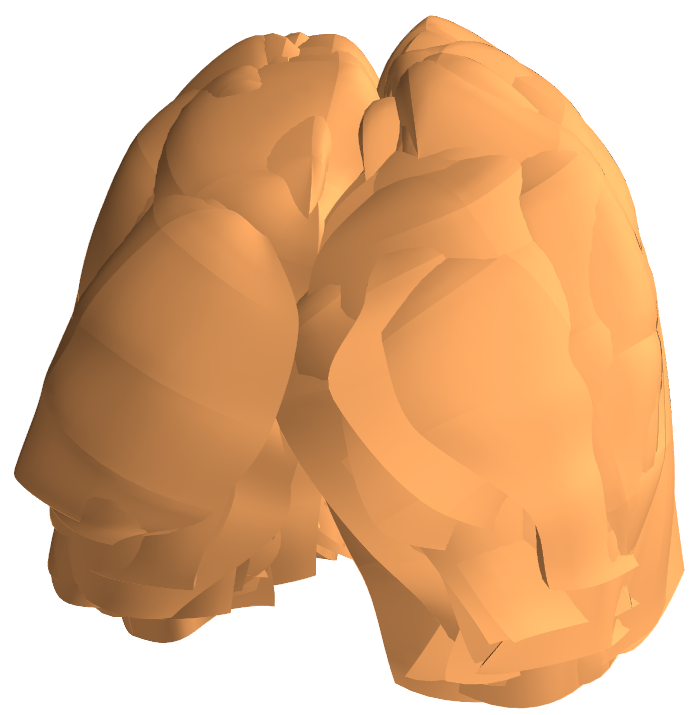
\includegraphics{Segmentation/Image/ProcrustedMeshes.png}}
  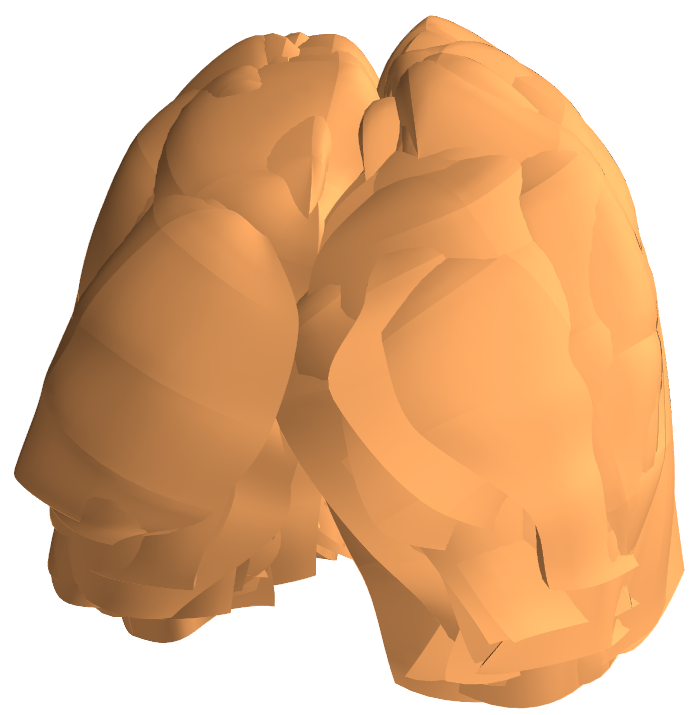
\includegraphics[width=\linewidth,trim={{.0\wd0} {.0\wd0} {.0\wd0} {.0\wd0}},clip]{Segmentation/Image/ProcrustedMeshes.png}
  \caption{}
  \label{fig:PCAMeshTraining-a} 
\end{subfigure}
%\vspace{.3in} % control space between the upper context and figure
\hspace{.3in} % control space between two figures
\begin{subfigure}{.4\linewidth}% set image scale
  \sbox0{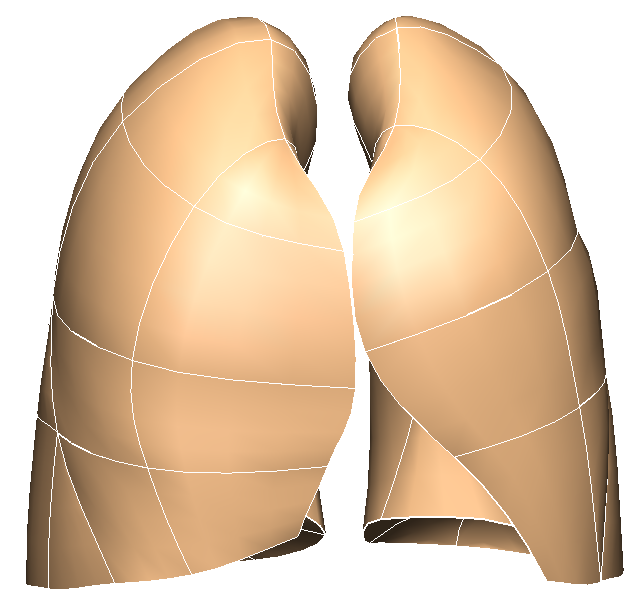
\includegraphics{Segmentation/Image/PCAAverageModel.png}}
  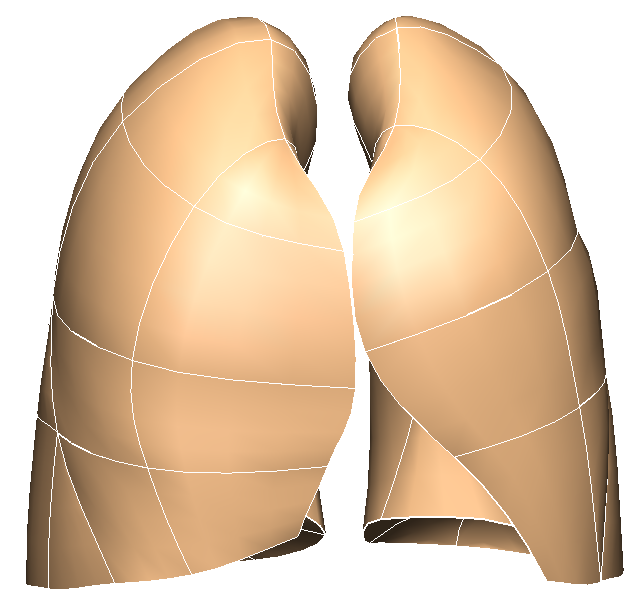
\includegraphics[width=\linewidth,trim={{.0\wd0} {.0\wd0} {.0\wd0} {.0\wd0}},clip]{Segmentation/Image/PCAAverageModel.png}
  \caption{}
  \label{fig:PCAMeshTraining-b} 
\end{subfigure}
\caption{Statistical shape model construction based on principal component analysis. (a) Procrustes aligned meshes of 50 subjects. (b) Average shape model of 50 training subjects. All the weight values are zero for this shape model.}
\label{fig:PCAMeshTraining}
\end{figure}

%%%%%%%%%%%%%%%%%%%%%%%%%%%%%%%%%%%%%%%%%%%%%%%%%%%%%%%
\subsection{Initial prediction of lobar location in an individual} \label{MeshPrediction}

Using the method described in section \ref{ShapeModelGeneration}, the lung shape variation across the training set can be decomposed into a series of modes, and each specific lung shape can be represented with the corresponding mode weight values. In this study each mode represents one type of lung and fissure surface shape variation. In order to predict the fissure location, two PCA-based SSMs were constructed using the same training dataset. The first lobe SSM was built using both the lung surface parameters and fissure surface parameters. The second lung SSM was derived for the same training set but did not include the fissure surfaces and so only described the shape of the lung surface.

The two SSMs were used to predict the fissure locations for subjects that were not part of the training set, using only the definition of the lung surface for the subject as input. A finite element mesh of the lung surface (without fissure information) was generated for each new subject. The new fitted lung mesh was procrustes aligned to the same reference model as the training subjects were aligned to. Then this aligned lung surface mesh was projected on to the lung surface SSM (with no fissure surfaces). The principal component weight values were calculated from the projection, which was represented as $w_{new} = [w_{new1}, w_{new2}, ..., w_{newL}]$ (L$\leq$ 49) here. The first seven principal components accounted for over 90\% of the total lung shape variation in the training set. Therefore, the first seven mode weights were used on the lobe SSM ( which includes both lung and fissure surfaces) to reconstruct the projected lobe mesh for this new subject

\begin{equation}
 \label{eq:FissurePrediction1}
 S_{new} = S_{mean} + \sum_{i=1}^7 \mathbf{u}_i w_{newi},
\end{equation}

\noindent where $S_{mean}$ is the average lobe shape model across all the subjects, $\mathbf{u}_i$ is the first seven eigenvectors of the covariance matrix C corresponding to the lobe \gls{ssm}, and $w_{newi}$ is the projected weight values from the lung \gls{ssm}. An initial estimation of fissure locations was then made (Figure \ref{fig:PCAFissurePrediction}). This initial prediction of lobar fissures provides a reduced search area for subsequent image analysis and ensures an estimation of complete lobar structures even if a fissure is incomplete or is difficult to detect.

\begin{figure}[htbp] 
\centering
\begin{subfigure}{.35\linewidth}% set image scale
  \sbox0{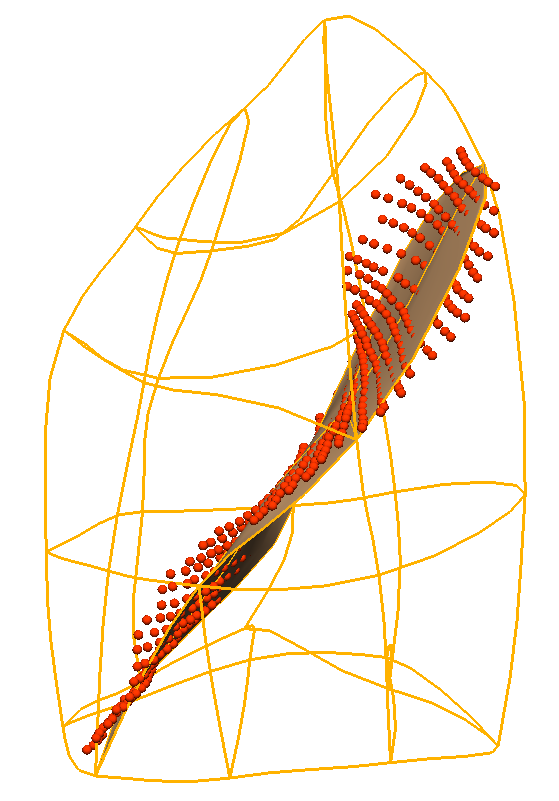
\includegraphics{Segmentation/Image/ProjectedLeftFissureMesh.png}}
  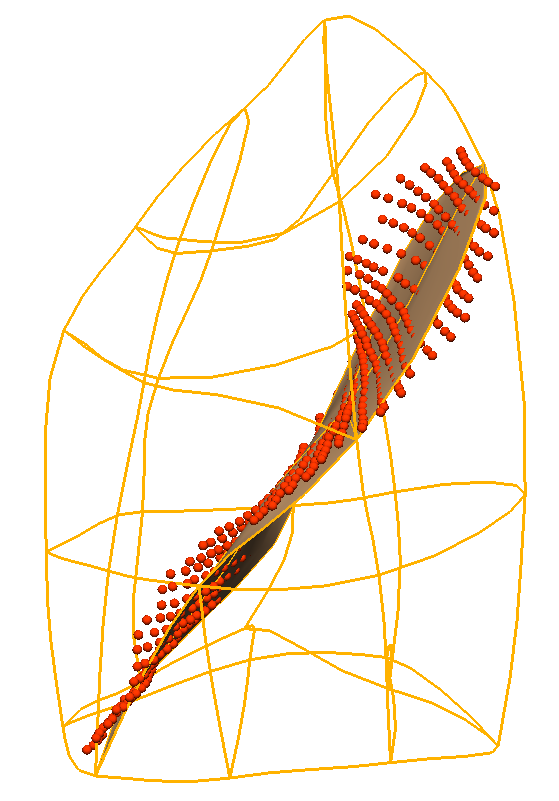
\includegraphics[width=\linewidth,trim={{.0\wd0} {.0\wd0} {.0\wd0} {.0\wd0}},clip]{Segmentation/Image/ProjectedLeftFissureMesh.png}
  \caption{}
  \label{fig:PCAFissurePrediction-a} 
\end{subfigure}
\begin{subfigure}{.37\linewidth}% set image scale
  \sbox0{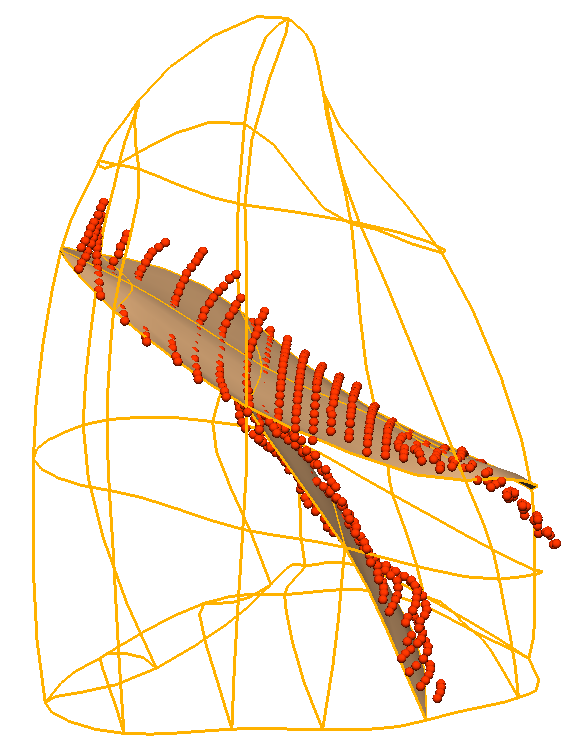
\includegraphics{Segmentation/Image/ProjectedRightFissureMesh.png}}
  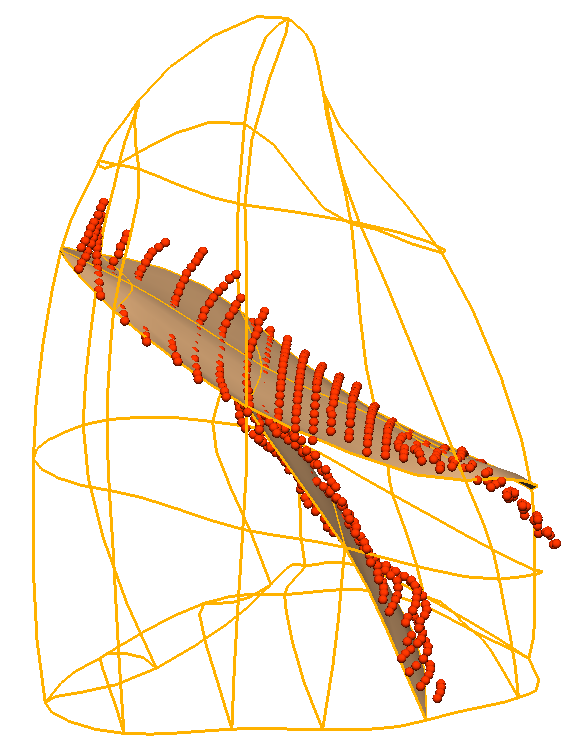
\includegraphics[width=\linewidth,trim={{.0\wd0} {.0\wd0} {.0\wd0} {.0\wd0}},clip]{Segmentation/Image/ProjectedRightFissureMesh.png}
  \caption{}
  \label{fig:PCAFissurePrediction-b} 
\end{subfigure}
\caption{Fissure prediction results compared to ground truth fissure points for one subject. The fissure surface meshes are estimated fissure locations and the red points are manual tracing fissure points by an expert. (a) Left lung. (b) Right lung.}
\label{fig:PCAFissurePrediction}
\end{figure}
%%%%%%%%%%%%%%%%%%%%%%%%%%%%%%%%%%%%%%%%%%%%%%%%%%%%%%%
\subsection{Multi-scale Hessian-based fissure detection}

The final fissure detection was accomplished using an enhancement filter. Conventional enhancement filters are typically based on first (structure tensor) or second (Hessian matrix) order image information \citep{frangi1998multiscale,lorenz1997multi}. This study used the Hessian matrix based on gray-scale curvature information combined with Gaussian smoothing as a basic operator to enhance the fissure structure. In 3D space, fissures are free-form surfaces in the lungs that locally resemble plate-like structures, since the grey-value increases rapidly from the structure border to the centre and decreases again to the opposite border. Hessian-based filters are typically used to enhance and differentiate structures with specific shapes, i.e., blobs, sheets and tubes \citep{frangi1998multiscale,lorenz1997multi}.

A common approach to analyse the local behaviour of an image, L, is to consider the local grey-value variations in the neighbourhood of a point $x_0$ modelled by a Taylor expansion to the second order

\begin{equation}
 \label{eq:FissureDetection1}
 L(x_o + \delta x_o, s) \approx L(x_o, s) + \delta{x_o}^T\nabla_{o,s} + \delta{x_o}^TH_{o,s}\delta x_o,
\end{equation}

\noindent where $\nabla_{o,s}$ and $H_{o,s}$ are the gradient vector and Hessian matrix, respectively, of the image computed in $x_o$ at scale s.

To calculate these differential operators of L, concepts of linear scale space theory are used \citep{koenderink1984structure,florack1992scale}. In this framework, differentiation is defined as a convolution with derivatives of Gaussians

\begin{equation}
 \label{eq:FissureDetection2}
 \pd{L(x,s)}{x} = s^\gamma L(x)*\pd{G(x,s)}{x},
\end{equation}

\noindent where the D-dimensional Gaussian is defined as

\begin{equation}
 \label{eq:FissureDetection3}
 G(x,s) = \frac{1}{{\sqrt{2\pi s^2}}^D}e^{-\frac{{\lVert x \rVert}^2}{2x^2}},
\end{equation}

\noindent where s is the kernel size of the Gaussian. The second derivative of a Gaussian is in many cases a good approximation to the optimal filter for a plane-like structure. Through using the second derivative operator combined with Gaussian smoothing as the basic operator (Hessian matrix), we are able to make the non-supervised fissure filter scale-dependent \citep{lorenz1997multi, li2003selective}. In order to make sure a variety of sizes of fissures can be captured by the Hessian, a range of kernel sizes was implemented from 0.5 mm to 2.5 mm in 0.5 mm increments as the kernel size of the Gaussian to obtain a final estimate of 'fissureness'

\begin{equation}
\label{eq:Multiscale}
F_{output} = \operatorname*{max}\limits_{s_{min}\leq s \leq s_{max}} F_0 (s),
\end{equation}

\noindent where $s_{min}$ and $s_{max}$ are the minimum scale (0.5 mm) and maximum scale (2.5 mm). Each scale s gets a response. In the final output of the multiscale enhancement filter, the maximum output over all scales is assigned to each voxel.

At each image voxel, the Hessian matrix was constructed from the six independent second order derivatives as a symmetric matrix

\begin{equation}
 \label{eq:FissureDetection4}
 Hessian = \begin{bmatrix} H_{xx} & H_{xy} & H_{xz} \\ H_{yx} & H_{yy} & H_{yz} \\ H_{zx} & H_{zy} & H_{zz} \\ \end{bmatrix},
\end{equation}

\noindent where $H_{ij} = \begin{vmatrix} \pd[2]{H}{r_i r_j} \\ \end{vmatrix}$, and r represents the gradient direction.

The idea behind eigenvalue analysis of the Hessian is to extract the principal directions in which the local second order structure of the image can be decomposed. The eigenvalue decomposition extracts three orthonormal directions which are invariant up to a scaling factor when mapped by the Hessian matrix. In this chapter, $\lambda_k$ will be the eigenvalue with the k-th smallest magnitude ($\mid\lambda_{1}\mid\leq\mid\lambda_{2}\mid\leq\mid\lambda_{3}\mid$). Under this assumption, Table \ref{tab:Hessian-based eigenvalue analysis} summarizes different structures distinguished by an analysis of the eigenvalues of the Hessian.

\begin{table}[h]
\centering
\caption{Possible structures on images in 2D and 3D, and its corresponding eigenvalues $\lambda_k$. H and L describe the absolute value of $\lambda_k$, H is high, L is low, +/- indicate the sign of the eigenvalue. The eigenvalues relationship here is: $\mid\lambda_{1}\mid\leq\mid\lambda_{2}\mid\leq\mid\lambda_{3}\mid$.}
\label{tab:Hessian-based eigenvalue analysis}
\begin{tabular}{c c | c c c | c}
\hline
\multicolumn{2}{c|}{\bf{2D}} & \multicolumn{3}{c|}{\bf{3D}} & \bf{Orientation structure}\\ 
\hline
$\lambda_1$ & $\lambda_2$ &  $\lambda_1$ & $\lambda_2$ & $\lambda_3$ &  \\
\hline
   L      &     L     &      L     &     L     &      L     & noisy structure \\
          &           &      L     &     L     &      H-    & bright plane-like structure \\
          &           &      L     &     L     &      H+    & dark plane-like structure \\
   L      &     H-    &      L     &     H-    &      H-    & bright tubular-like structure \\
   L      &     H+    &      L     &     H+    &      H+    & dark tubular-like structure \\
   H-     &     H-    &      H-    &     H-    &      H-    & bright blob-like structure \\	
   H+     &     H+    &      H+    &     H+    &      H+    & dark blob-like structure \\												
\hline
\end{tabular}
\end{table}

As shown in Table \ref{tab:Hessian-based eigenvalue analysis}, an eigenvector analysis of the Hessian matrix can thus be used to detect fissure-like structures, and the respective eigenvectors point out singular directions. In 3D space, a light plane on a dark background is characterized by one large positive second derivative ($\lambda_3$) perpendicular to the fissure plane, since the grey-value increases rapidly from the plane-structure border to the centreline and decreases again to the opposite border. And two small second derivatives of either sign ($\lambda_1$ and $\lambda_2$) parallel to the plane should occur (shown in Fig \ref{fig:FissureHessianEigenvector}). Thus, on the bright fissures, the ideal relationship is defined as $\mid\lambda_{1}\mid = \mid\lambda_{2}\mid = 0$ and $\lambda_{3} \ll 0$, $\mid\lambda_{1}\mid\leq\mid\lambda_{2}\mid\leq\mid\lambda_{3}\mid$. From these characteristics, we can get a fissure probability of each voxel defined as

\begin{equation}
\label{eq:FissureHessian1}
F_0(s) = \Theta S_{plane} S_{noise}.
\end{equation}

The parameter $\Theta$ supresses points whose largest eigenvalue $\lambda_{3}$ is positive, since fissures are locally bright , and is defined as

\begin{equation}
\label{eq:FissureHessian2}
\Theta = \begin{cases}
         1,\quad \lambda_{3}< 0\\,
         0, \quad \lambda_{3}\geq0.
         \end{cases}
\end{equation}

Since the largest eigenvalue $\mid\lambda_{3}\mid$ should be much larger than the other two eigenvectors, the second factor $S_{plane}$ uses the ratio between $\mid\lambda_{2}\mid$ and $\mid\lambda_{3}\mid$ to search sheet-like structures, so that the voxels where $\mid\lambda_{3}\mid$ and $\mid\lambda_{2}\mid$ are significantly different. $S_{plane}$ is defined as

\begin{equation}
\label{eq:FissureHessian3}
S_{plane} = exp(-\frac{{R_{plane}}^2}{2\alpha^2}), \\
\end{equation}

\begin{equation}
\label{eq:FissureHessian4}
R_{plane} = \frac{\mid\lambda_{2}\mid}{\mid\lambda_{3}\mid},
\end{equation}

\noindent where $\alpha$ was set to 0.5 in this study. The third factor $S_{noise}$ aims to suppress noise voxels such as blob-like structures. Unlike plane-like structures which have relatively large $\mid\lambda_{2}\mid$ and $\mid\lambda_{3}\mid$ ratio, the noise voxels usually have low $\mid\lambda_{1}\mid$, $\mid\lambda_{2}\mid$ and $\mid\lambda_{3}\mid$ (as shown in Table \ref{tab:Hessian-based eigenvalue analysis}). Therefore, here we use

\begin{equation}
\label{eq:FissureHessian5}
S_{noise} = 1 - exp(-\frac{{R_{noise}}^2}{2\beta^2}), \\
\end{equation}

\begin{equation}
\label{eq:FissureHessian6}
R_{noise} = \sqrt{{\lambda_1}^2+{\lambda_2}^2+{\lambda_3}^2},
\end{equation}

\noindent with $\beta$ set to 0.5 for thresholding. $F_0(s)$ then gives a high response to local plane-like structures (fissures) and suppresses other pulmonary structures (noise). An example of this enhancement filter applied in an individual is shown in Figure \ref{fig:FissureDetection-a}. 

\begin{figure*}[htbp]
  \centering 
	\vspace{.15in} % control space between the upper context and figure
  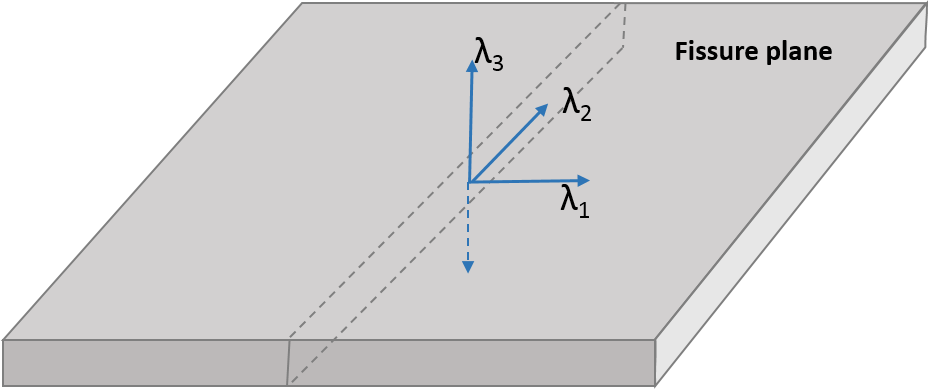
\includegraphics[height=1.5in]{Segmentation/Image/FissureHessianEigenvector.png}
  \caption{The three eigenvectors of the Hessian matrix representing plane-like structure (fissure). $\lambda_1$ and $\lambda_2$ are parallel to fissure plane, $\lambda_3$ is perpendicular to fissure plane.}
  \label{fig:FissureHessianEigenvector}
\end{figure*}

Blood vessel voxels were subsequently filtered from the fissure enhanced result. The segmentation of vessels was achieved using a classical vessel segmentation method \citep{frangi1998multiscale}. This method uses a multiple scale (from 0.5 mm to 3.0 mm in 0.5 mm increments as the kernel size of Gaussian) Hessian-based enhanced filter, which is similar to the fissure detection filter described previously. The main difference is here the aim is to search for the tube structure (vessels). In a 3D image,  the relationship of Hessian eigenvalues $\lambda_{1}$, $\lambda_{2}$ and $\lambda_{3}$ of an ideal bright tubular structure in a dark background should be described as $\mid\lambda_{1}\mid\approx$ 0, $\mid\lambda_{1}\mid\ll\mid\lambda_{2}\mid$,  $\lambda_{2}\approx\lambda_{3}$ (see Figure \ref{fig:VesselHessianEigenvector}). Therefore, the following equations were used as the enhancement filter to detect vesselness structures

\begin{equation}
\label{eq:VesselHessian1}
V_0(s) = \begin{cases}
         0,\quad\quad\quad\quad\quad\quad\quad if \quad \lambda_{2}>0,\\
         (1-exp(-\frac{{R_A}^2}{a^2}))exp(-\frac{{R_B}^2}{2b^2})(1-exp(-\frac{S^2}{2c^2})),
         \end{cases}
\end{equation}

\noindent where a and b were both set to 0.5, and c was set to 500 in this study. $R_A$, $R_B$ and S are defined as

\begin{equation}
\label{eq:VesselHessian2}
R_A = \frac{\mid\lambda_{2}\mid}{\mid\lambda_{3}\mid}, 
\end{equation}

\begin{equation}
\label{eq:VesselHessian3}
R_B = \frac{\mid\lambda_{1}\mid}{\sqrt{\mid\lambda_{2}\mid \mid\lambda_{3}\mid}},
\end{equation}

\begin{equation}
\label{eq:VesselHessian3}
S = {\Vert H \rVert}_F = \sqrt{\sum_{j\leq D}}{\lambda_j}^2,
\end{equation}

\noindent where $D$ is the dimension of the image. $V_0(s)$ gives a probability of vesselness for each voxel. Then segmented blood vessels were selected through detecting the voxels whose vesselness value was larger than a specific threshold (threshold = 10 in this study \citep{frangi1998multiscale}). $D{vessel}$ was used to represent the distance transform to the segmented vessel line, thus the final fissureness after decreasing the values of vessel voxels was defined as

\begin{equation}
\label{eq:FinalFissureness}
F_{final}(s) = F_0(s)S_{vessels},
\end{equation}

\begin{equation}
\label{eq:FinalFissureness}
S_{vessels} = exp(1-\frac{{D{vessel}}^2}{2d^2}),
\end{equation}

\noindent  where $d$ was set to 5mm in this study. High vesselness voxels were therefore suppressed and not detected as fissure points in the final result. Fig \ref{fig:FissureDetection-b} shows the result after eliminating the vessel voxels.

\begin{figure*}[htbp]
  \centering 
  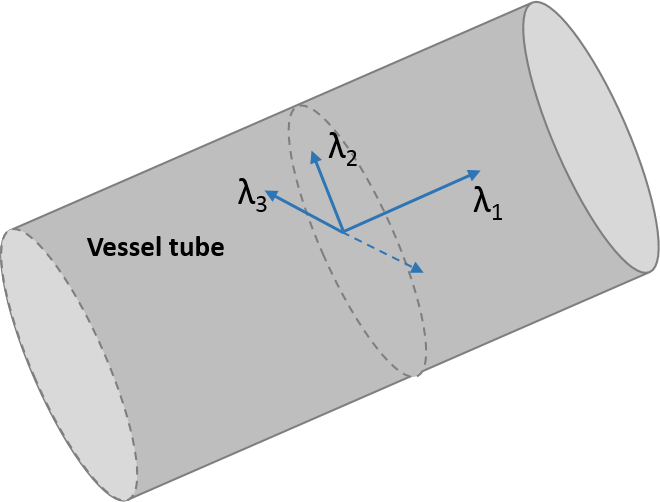
\includegraphics[height=1.5in]{Segmentation/Image/VesselHessianEigenvector.png}
  \caption{The three eigenvectors of the Hessian matrix representing tube-like structure (vessel). $\lambda_1$ is parallel to vessel tube, $\lambda_2$  and $\lambda_3$ are perpendicular to vessel tube.}
  \label{fig:VesselHessianEigenvector}
\end{figure*}

The initial fissure location predicted by average SSM deformation gives a region of interest (ROI) for an accurate fissure detection, see Figure \ref{fig:FissureDetection-c}. The candidate points are selected within a certain distance of the initial fissure approximation: the search distance was set to 20 voxels (default value) for the initially projected left and right oblique fissures and 15 voxels for the initially projected right horizontal fissure. To remove some spurious responses such as small plane-like structures on the result, a 2D 4-neighbourhood connected component filter and a 3D 6-neighbourhood vector-based connected component filter were employed successively to eliminate noise arising from small plane-like structures in this search region (Fig \ref{fig:FissureDetection-d}). A 2D filter was used to eliminate 4-neighbour connected components that were smaller than a minimum small size (set to 10 voxels initially) slice by slice. The 3D vector-based connected component filter used the inner product of the normalized largest eigenvector of the Hessian matrix in adjacent voxels. These largest eigenvectors are perpendicular to the fissure plane, and their inner product provides a criterion for component connection. As the curvature of a fissure is locally low, adjacent fissure voxels should have similar largest eigenvectors and thus the inner product value of their largest eigenvectors should equal to 1 or slightly smaller than 1. Connected boundary condition was set as an inner product $\leq$ 0.8 to connected component, then 3D 6-neighbour connected component with a volume less than 100 $\mathrm{mm^3}$ was removed as noise from the result.

The detected points were then divided into a set of small subsections corresponding to different x, y intervals. For each subsection, the point of the highest fissure probability (the highest S value) was selected as the final candidate fissure point (Fig \ref{fig:FissureDetection-e}). Once the maximum fissureness candidates were found, a morphological dilation with a $3\times3\times3$ voxel cube as structure element was applied iteratively until the largest connected fissure plane was big enough, so that all the other unconnected outliers could be filtered subsequently. Finally, a continuous smooth fissure surface was generated based on the maximum fissure points using a $\beta$-spline method with a thin-plane spline \citep{lee1997scattered} and extrapolated to the lung boundaries, see Fig \ref{fig:FissureDetection-f}.

\begin{figure}[htbp] 
\centering
\begin{subfigure}{.41\linewidth}% set image scale
  \sbox0{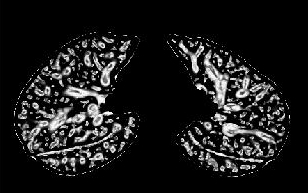
\includegraphics{Segmentation/Image/FissureDetection1.jpg}} 
  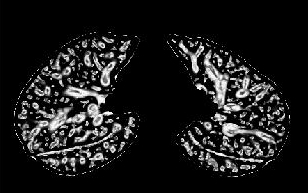
\includegraphics[width=\linewidth,trim={{.0\wd0} {.0\wd0} {.0\wd0} {.0\wd0}},clip]{Segmentation/Image/FissureDetection1.jpg} %trim={<left> <lower> <right> <upper>}, set the cut scale
  \caption{}
	\label{fig:FissureDetection-a}
\end{subfigure} 
\begin{subfigure}{.408\linewidth}% set image scale
  \sbox0{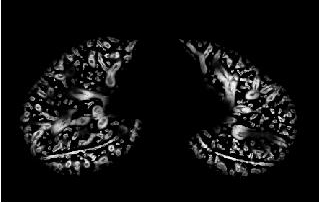
\includegraphics{Segmentation/Image/FissureDetection2.jpg}}
  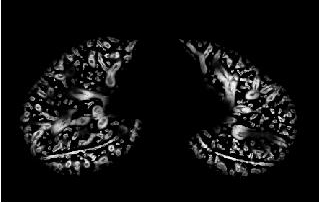
\includegraphics[width=\linewidth,trim={{.0\wd0} {.0\wd0} {.0\wd0} {.0\wd0}},clip]{Segmentation/Image/FissureDetection2.jpg}
  \caption{}
	\label{fig:FissureDetection-b}
\end{subfigure}
\begin{subfigure}{.4\linewidth}% set image scale
  \sbox0{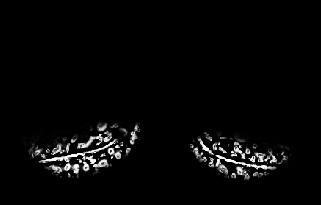
\includegraphics{Segmentation/Image/FissureDetection3.jpg}}
  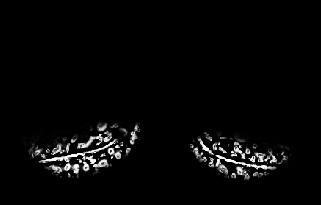
\includegraphics[width=\linewidth,trim={{.0\wd0} {.0\wd0} {.0\wd0} {.0\wd0}},clip]{Segmentation/Image/FissureDetection3.jpg}
  \caption{}
	\label{fig:FissureDetection-c}
\end{subfigure}
\begin{subfigure}{.412\linewidth}% set image scale
  \sbox0{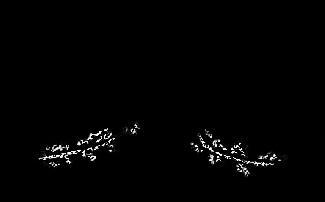
\includegraphics{Segmentation/Image/FissureDetection4.jpg}}
  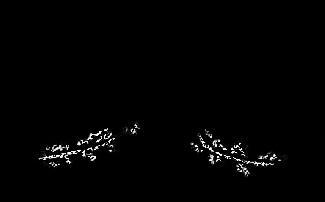
\includegraphics[width=\linewidth,trim={{.0\wd0} {.0\wd0} {.0\wd0} {.0\wd0}},clip]{Segmentation/Image/FissureDetection4.jpg}\label{fig:FissureDetection}
  \caption{}
	\label{fig:FissureDetection-d}
\end{subfigure}
\begin{subfigure}{.41\linewidth}% set image scale
  \sbox0{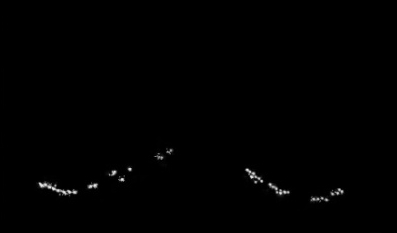
\includegraphics{Segmentation/Image/FissureDetection5.jpg}}
  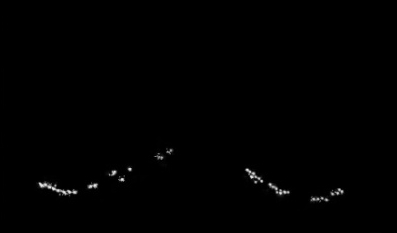
\includegraphics[width=\linewidth,trim={{.0\wd0} {.0\wd0} {.0\wd0} {.0\wd0}},clip]{Segmentation/Image/FissureDetection5.jpg}
  \caption{}
	\label{fig:FissureDetection-e}
\end{subfigure}
\begin{subfigure}{.415\linewidth}% set image scale
  \sbox0{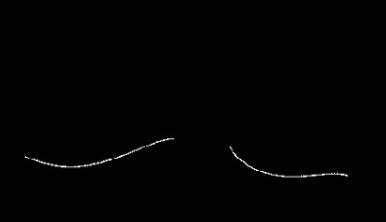
\includegraphics{Segmentation/Image/FissureDetection6.jpg}}
  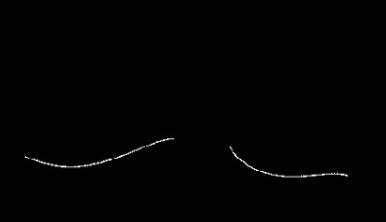
\includegraphics[width=\linewidth,trim={{.0\wd0} {.0\wd0} {.0\wd0} {.0\wd0}},clip]{Segmentation/Image/FissureDetection6.jpg}
  \caption{}
	\label{fig:FissureDetection-f}
\end{subfigure}
\caption{Hessian-based multiscale fissure detection results. (a) Hessian-based plane-like structure enhancement filter. (b) Remove vessel voxels (tube-like structures). (c) Selected search regions for fissure detection based on SSM initial fissure prediction. (d) 2D and 3D eigenvector based connected component filter. (e) Fissure candidate points. (f) $\beta$-spline curve fissure surface fitting.}
\label{fig:FissureDetection}
\end{figure}

%%%%%%%%%%%%%%%%%%%%%%%%%%%%%%%%%%%%%%%%%%%%%%%%%%%%%%%%
\subsection{Interactive user control interface} \label{UserControl}
As discussed above, a series of parameter values need to be chosen correctly to ensure a successful lobar segmentation. However, a fixed parameter value is usually not suitable for all the subjects due to a wide variation of lung tissue and fissure appearances across the population. Therefore, a fast and convenient manual interaction to control the segmentation procedure is reasonable and acceptable. Based on an open source software, Pulmonary Toolkit (PTK, https://github.com/tomdoel/pulmonarytoolkit), an improved user-friendly interactive interface was developed to control the segmentation parameters as input (improved version: https://github.com/qiuyufly/pulmonarytoolkit/tree/yuwen). PTK is a software developed on Matlab for the analysis of 3D medical lung images for academic research use. It comprises a library of lung analysis algorithms, a GUI application for visualising and analysing clinical lung images and a rapid prototyping framework for users to develop their new algorithms in an easy way. By making use of some built-in objects and the visualisation system of PTK, the lobar segmentation algorithm was added into the algorithm package and parameter control buttons were made available on the interface. Table \ref{tab:ParameterUserControl} summarises the interactive user control parameters. Figure \ref{fig:PTKUserInterface} shows the user interface of PTK.

\newcolumntype{C}[1]{>{\centering\arraybackslash}p{#1}}
\begin{table}[htbp]
\centering
\caption{Summary of interactive user control parameters}
\label{tab:ParameterUserControl}
\begin{tabular}{|p{4.5cm}|p{2.3cm}|l|}
\hline
\bf{Parameters} & \bf{Default values} & \bf{Notes}\\ 
\hline
Search region for left oblique fissure & 20 voxels &  \multirow{3}{5.2cm}{Increase the value if there are not enough positive candidate points; decrease the value if there is too much noise} \\
\cline{1-2}
Search region for right horizontal fissure & 20 voxels &  ~ \\
\cline{1-2}
Search region for right oblique fissure & 15 voxels &  ~ \\
\hline
Connected component size for left oblique fissure & 30 voxels &  \multirow{4}{5.2cm}{Decrease the value if there are\\not enough positive candidate points; increase the value if there is too much noise} \\
\cline{1-2}
Connected component size for right horizontal fissure & 30 voxels &  ~ \\
\cline{1-2}
Connected component size for right oblique fissure & 30 voxels &  ~ \\
\cline{1-2}
Total connected component size & 300 voxels &  ~ \\
\hline
\end{tabular}
\end{table}

\begin{figure*}[htbp]
  \flushleft 
  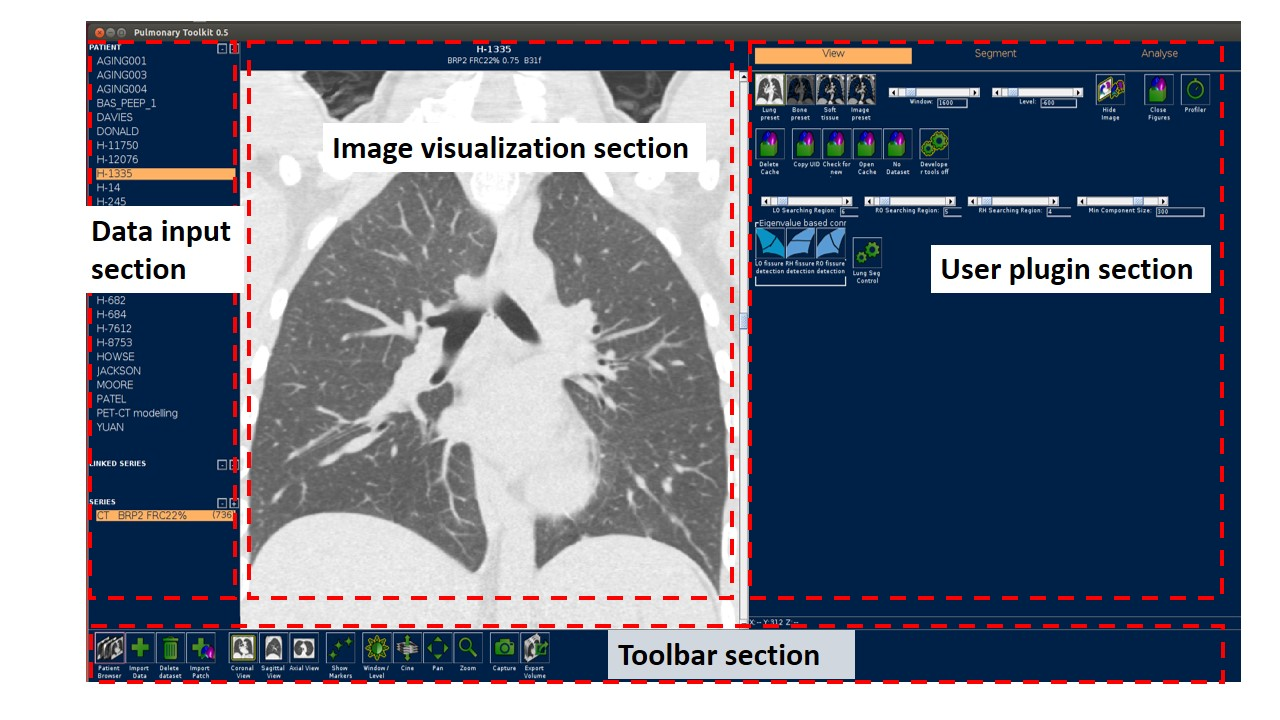
\includegraphics[height=3.2in]{Segmentation/Image/PTKUserInterface.jpg}
  \caption{PTK User interactive interface. It consists of data input section, image visualization section, user plugin section and toolbar section.}
  \label{fig:PTKUserInterface}
\end{figure*}

%%%%%%%%%%% 
\subsubsection{Search region control}
Fissure candidate points were detected within a certain distance of the initial fissure approximation. The default distance was set to 20 voxels for left and right oblique fissures and 15 voxels for right horizontal fissure. However, with a fixed search distance, fissure detection sometimes could not be implemented efficiently and accurately. The probability of error detection may increase if the search distance is too large, as more noise will be included in the initial search region. In contrast some positive fissure points will be missed if the search distance is too small. Accurate fissure candidate points are an important prerequisite for good fissure surface fitting. Therefore, user interactive slide buttons were developed on the PTK interface to control the search distance. Through inputting SSM based initial fissure prediction mesh, the estimated fissures can be  visualized to overlap on the raw images in the PTK visualization section. Then it is possible for users to select a suitable search region for each fissure depending on the accuracy of the initial fissure estimate. The better the initial fissure approximation, the lower the search region that should be selected. Figure \ref{fig:SearchRegionControl} shows the lobe segmentation result before and after change to the search region.
\newpage

\begin{figure}[htbp] 
\centering
\begin{subfigure}{.32\linewidth}% set image scale
  \sbox0{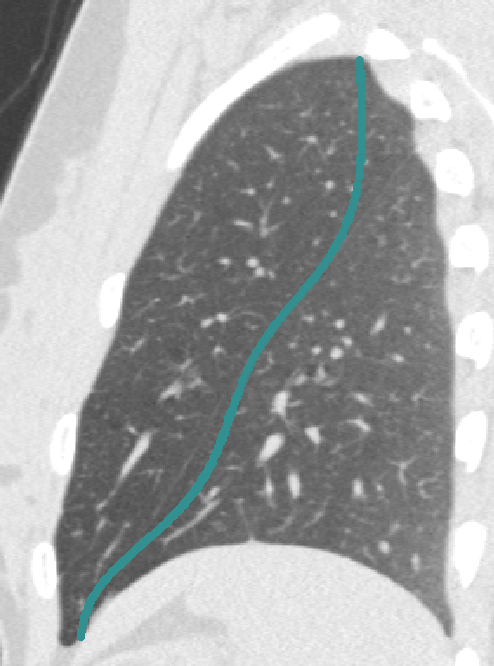
\includegraphics{Segmentation/Image/BeforeChangeSearchRegion.png}}
  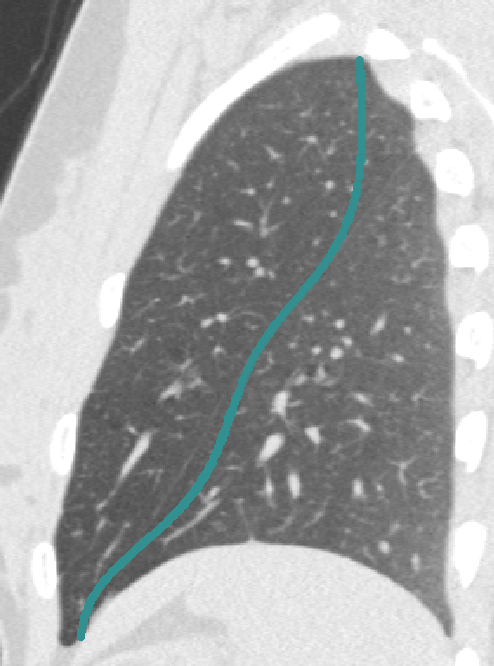
\includegraphics[width=\linewidth,trim={{.0\wd0} {.0\wd0} {.0\wd0} {.0\wd0}},clip]{Segmentation/Image/BeforeChangeSearchRegion.png}
  \caption{}
  \label{fig:SearchRegionControl-a} 
\end{subfigure}
%\vspace{.3in} % control space between the upper context and figure
\hspace{.3in} % control space between two figures
\begin{subfigure}{.33\linewidth}% set image scale
  \sbox0{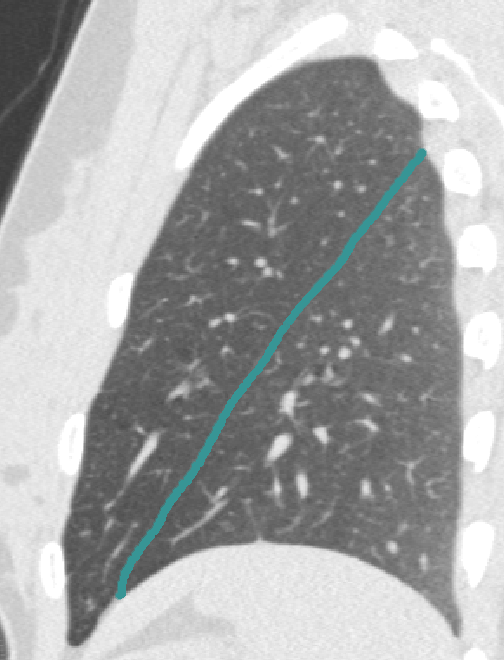
\includegraphics{Segmentation/Image/AfterChangeSearchRegion.png}}
  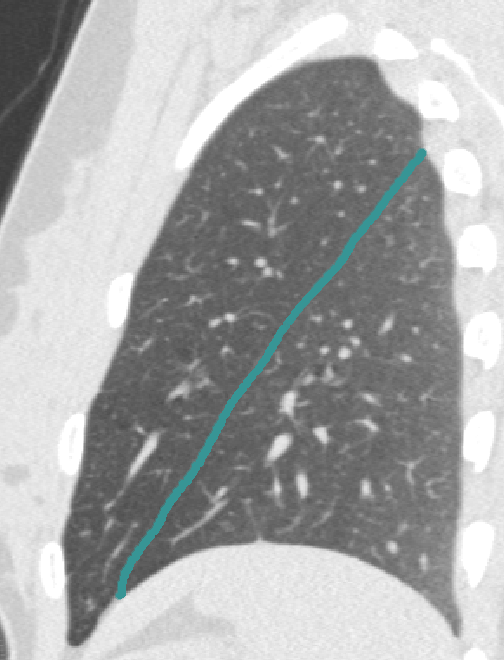
\includegraphics[width=\linewidth,trim={{.0\wd0} {.0\wd0} {.0\wd0} {.0\wd0}},clip]{Segmentation/Image/AfterChangeSearchRegion.png}
  \caption{}
  \label{fig:SearchRegionControl-b} 
\end{subfigure}
\caption{Fissure detection results before and after control the search regions. (a) Fissure detection result with a search distance of default 20 voxels. (b) Fissure detection result after setting a specific search distance depending on the accuracy of initial fissure guessing.}
\label{fig:SearchRegionControl}
\end{figure}

\subsubsection{Connected component analysis filter control}
Connected component analysis is an important operation to help with noise elimination during fissure detection. A suitable connected component size is able to remove most of the small connected structures as outliers and in the meantime retain true fissure structures as much as possible. In order to improve the filter performance, a slide button was used to control the connected component size on the PTK user interface. Through changing the component size threshold, it is possible for us to find a balance between spurious response elimination and target points retainment. 

\subsubsection{Manual correction}
Manual correction remains an essential part of lobe segmentation processing. A manual correction tool was available in the PTK software, but in this method only one correct landmark could be selected at a time. Here, a multiple landmark correction method was developed based on PTK built-in packages, and the improved correction tool allows users to modify three fissure points at the same time. By selecting a series of correction landmarks, the corresponding fissure plane is deformed to a new curved surface which passes through all the correct landmarks. The correction region was calculated based on the distance between the landmark and its corresponding fissure plane, and a 3D Gaussian filter with the landmark as the centre was also used to specify the corrected boundary. The correction happens in 3D space so that users don't need to do the correction slice by slice. The whole correction can be finished in a few minutes even when automatic fissure is not complete. Figure \ref{fig:ManualCorrection} shows the fissure detection results before and after manual correction.

\begin{figure}[htbp] 
\centering
\begin{subfigure}{.44\linewidth}% set image scale
  \sbox0{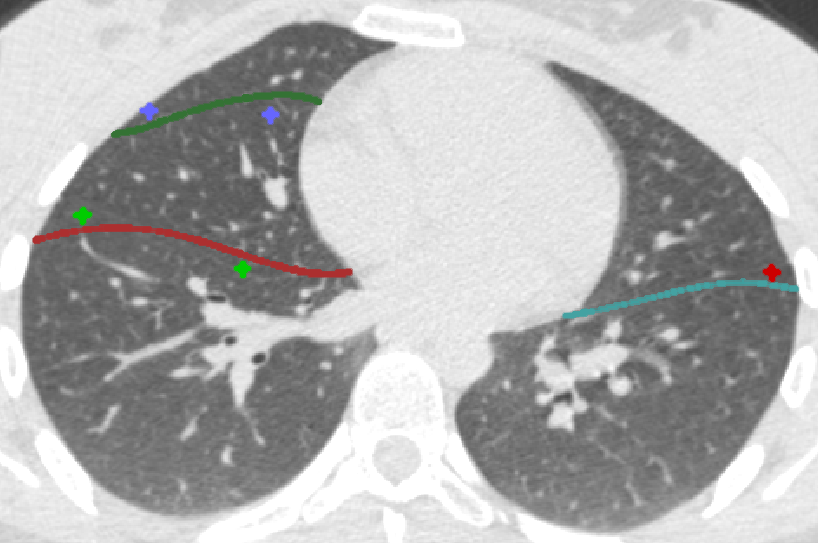
\includegraphics{Segmentation/Image/BeforeManualCorrection.png}}
  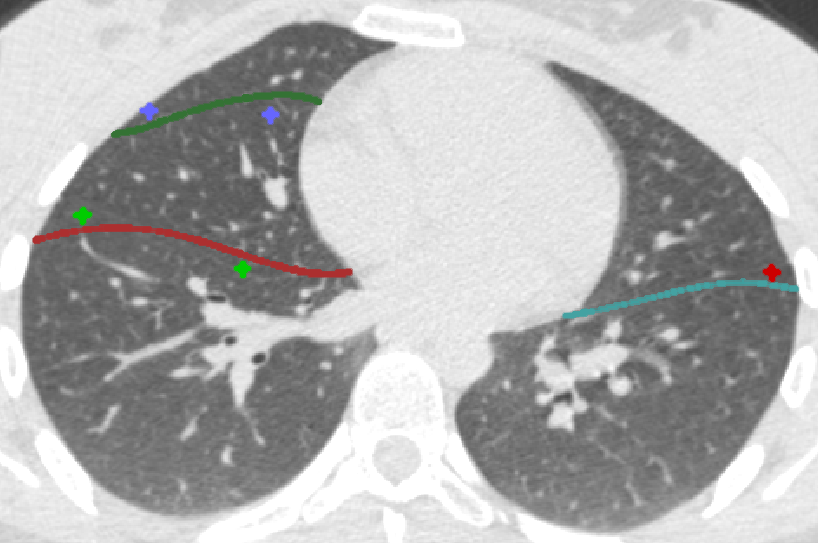
\includegraphics[width=\linewidth,trim={{.0\wd0} {.0\wd0} {.0\wd0} {.0\wd0}},clip]{Segmentation/Image/BeforeManualCorrection.png}
  \caption{}
  \label{fig:ManualCorrection-a} 
\end{subfigure}
\vspace{.1in} % control space between the upper context and figure
%\hspace{.3in} % control space between two figures
\begin{subfigure}{.44\linewidth}% set image scale
  \sbox0{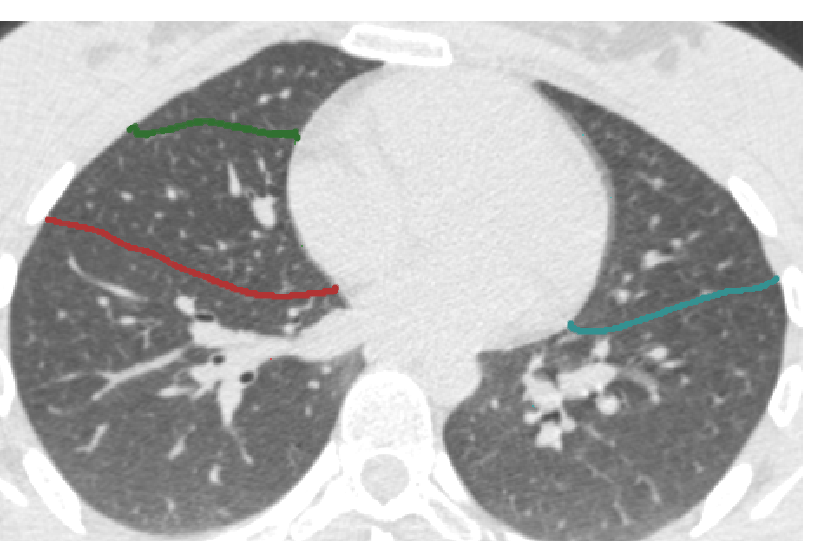
\includegraphics{Segmentation/Image/AfterManualCorrection.png}}
  \includegraphics[width=\linewidth,trim={{.0\wd0} {.0\wd0} {.0\wd0} {.0\wd0}},clip]{Segmentation/Image/AfterManualCorrection.png}
  \caption{}
  \label{fig:ManualCorrection-b} 
\end{subfigure}
\caption{Manual correction on automatic fissure detection results (a) Manually select a set of landmarks on real fissure lines shown in raw images to correct automatic fissure detection results (red landmarks are for left oblique fissure, green landmarks are for right oblique fissure, blue landmarks are for right horizontal fissure). (b) Corrected fissure detection results shown with raw images. The corrected fissure lines can match the real fissure locations.}
\label{fig:ManualCorrection}
\end{figure}

%%%%%%%%%%%%%%%%%%%%%%%%%%%%%%%%%%%%%%%%%%%%%%%%%%%%%%%
\section{Results for SMM segmentation} \label{SegmentationExperiment}

\subsection{Testing CT dataset}
The semi-automatic SSM lobe segmentation method was tested on two datasets: 1) CT images from five young normal subjects taken at different lung volumes (end inspiration and end expiration), in the supine posture, from the HLA dataset (introduced in Section \ref{ShapeModelGeneration}). The selected dataset consists of five end expiration images and five end inspiration images, which were not part of the SSM training set; 2) CT images from older patients (slice thickness 1.25-3.00 mm) acquired during routine diagnostic inspection for idiopathic pulmonary fibrosis (IPF). Data from these subjects were acquired from the \gls{adhb}. Access to clinical data was approved by the Southern Health and Disability Ethics Committee. 

\subsection{Test and results}
Figure \ref{fig:HLASegmentationResults} shows raw images, initial SSM based fissure predicted locations, and the final automatic SSM-based lobar segmentation results (no manual correction) for a normal healthy subject. Figure \ref{fig:IPFSegmentationResults} shows the results for an IPF subject.

\begin{figure}[htbp] 
\centering
\begin{subfigure}{.25\linewidth}% set image scale
  \sbox0{\includegraphics{Segmentation/Image/H1335_FRC_Raw_Sagittal.png}}
  \begin{overpic}[width=\linewidth,trim={{.0\wd0} {.0\wd0} {.0\wd0} {.0\wd0}},clip]{Segmentation/Image/H1335_FRC_Raw_Sagittal.png}
      \put(16,105){\bf{Raw images}}
			\put(-38,55){\bf{Sagittal}}
  \end{overpic}
  \caption{}
  \label{fig:HLASegmentationResults-a} 
\end{subfigure}
%\vspace{.1in} % control space between the upper context and figure
\hspace{.3in} % control space between two figures
\begin{subfigure}{.25\linewidth}% set image scale
  \sbox0{\includegraphics{Segmentation/Image/H1335_FRC_PCAInitial_Sagittal.png}}
  \begin{overpic}[width=\linewidth,trim={{.0\wd0} {.0\wd0} {.0\wd0} {.0\wd0}},clip]{Segmentation/Image/H1335_FRC_PCAInitial_Sagittal.png}
      \put(0,105){\bf{Initial SSM-based fissures}}
  \end{overpic}
  \caption{}
  \label{fig:HLASegmentationResults-b} 
\end{subfigure}
%\vspace{.1in} % control space between the upper context and figure
\hspace{.3in} % control space between two figures
\begin{subfigure}{.25\linewidth}% set image scale
  \sbox0{\includegraphics{Segmentation/Image/H1335_FRC_PCAFissureDetection_Sagittal.png}}
  \begin{overpic}[width=\linewidth,trim={{.0\wd0} {.0\wd0} {.0\wd0} {.0\wd0}},clip]{Segmentation/Image/H1335_FRC_PCAFissureDetection_Sagittal.png}
      \put(15,105){\bf{Final fissures}}
  \end{overpic}
  \caption{}
  \label{fig:HLASegmentationResults-c} 
\end{subfigure}
\begin{subfigure}{.32\linewidth}% set image scale
  \sbox0{\includegraphics{Segmentation/Image/H1335_FRC_Raw_Axial.png}}
  \begin{overpic}[width=\linewidth,trim={{.0\wd0} {.0\wd0} {.0\wd0} {.0\wd0}},clip]{Segmentation/Image/H1335_FRC_Raw_Axial.png}
			\put(-30,30){\bf{Axial}}
  \end{overpic}
  \caption{}
  \label{fig:HLASegmentationResults-d} 
\end{subfigure}
%\vspace{.1in} % control space between the upper context and figure
%\hspace{.3in} % control space between two figures
\begin{subfigure}{.32\linewidth}% set image scale
  \sbox0{\includegraphics{Segmentation/Image/H1335_FRC_PCAInitial_Axial.png}}
  \includegraphics[width=\linewidth,trim={{.0\wd0} {.0\wd0} {.0\wd0} {.0\wd0}},clip]{Segmentation/Image/H1335_FRC_PCAInitial_Axial.png}
  \caption{}
  \label{fig:HLASegmentationResults-e} 
\end{subfigure}
%\vspace{.1in} % control space between the upper context and figure
%\hspace{.3in} % control space between two figures
\begin{subfigure}{.32\linewidth}% set image scale
  \sbox0{\includegraphics{Segmentation/Image/H1335_FRC_PCAFissureDetection_Axial.png}}
  \includegraphics[width=\linewidth,trim={{.0\wd0} {.0\wd0} {.0\wd0} {.0\wd0}},clip]{Segmentation/Image/H1335_FRC_PCAFissureDetection_Axial.png}
  \caption{}
  \label{fig:HLASegmentationResults-f} 
\end{subfigure}
\begin{subfigure}{.32\linewidth}% set image scale
  \sbox0{\includegraphics{Segmentation/Image/H1335_FRC_Raw_Coronal.png}}
  \begin{overpic}[width=\linewidth,trim={{.0\wd0} {.0\wd0} {.0\wd0} {.0\wd0}},clip]{Segmentation/Image/H1335_FRC_Raw_Coronal.png}
			\put(-35,40){\bf{Coronal}}
  \end{overpic}
  \caption{}
  \label{fig:HLASegmentationResults-g} 
\end{subfigure}
%\vspace{.1in} % control space between the upper context and figure
%\hspace{.3in} % control space between two figures
\begin{subfigure}{.32\linewidth}% set image scale
  \sbox0{\includegraphics{Segmentation/Image/H1335_FRC_PCAInitial_Coronal.png}}
  \includegraphics[width=\linewidth,trim={{.0\wd0} {.0\wd0} {.0\wd0} {.0\wd0}},clip]{Segmentation/Image/H1335_FRC_PCAInitial_Coronal.png}
  \caption{}
  \label{fig:HLASegmentationResults-h} 
\end{subfigure}
%\vspace{.1in} % control space between the upper context and figure
%\hspace{.3in} % control space between two figures
\begin{subfigure}{.32\linewidth}% set image scale
  \sbox0{\includegraphics{Segmentation/Image/H1335_FRC_PCAFissureDetection_Coronal.png}}
  \includegraphics[width=\linewidth,trim={{.0\wd0} {.0\wd0} {.0\wd0} {.0\wd0}},clip]{Segmentation/Image/H1335_FRC_PCAFissureDetection_Coronal.png}
  \caption{}
  \label{fig:HLASegmentationResults-i} 
\end{subfigure}
\caption{Sagittal, axial, and coronal views illustrating raw image, SSM based initial fissure guessing and final automatic fissure detection results of a normal healthy subject. (a), (d), (g) are sagittal, axial and coronal raw images. (b), (e), (h) are sagittal, axial and coronal SSM based initial fissure guessing results. (c), (f), (i) are sagittal, axial and coronal automatic fissure detection results.}
\label{fig:HLASegmentationResults}
\end{figure}

\begin{figure}[htbp] 
\centering
\begin{subfigure}{.25\linewidth}% set image scale
  \sbox0{\includegraphics{Segmentation/Image/IPF203_Raw_Sagittal161.png}}
  \begin{overpic}[width=\linewidth,trim={{.0\wd0} {.0\wd0} {.0\wd0} {.0\wd0}},clip]{Segmentation/Image/IPF203_Raw_Sagittal161.png}
      \put(16,105){\bf{Raw images}}
			\put(-45,55){\bf{Sagittal}}
  \end{overpic}
  \caption{}
  \label{fig:IPFSegmentationResults-a} 
\end{subfigure}
%\vspace{.1in} % control space between the upper context and figure
\hspace{.3in} % control space between two figures
\begin{subfigure}{.25\linewidth}% set image scale
  \sbox0{\includegraphics{Segmentation/Image/IPF203_PCAGuessing_Sagittal161.png}}
  \begin{overpic}[width=\linewidth,trim={{.0\wd0} {.0\wd0} {.0\wd0} {.0\wd0}},clip]{Segmentation/Image/IPF203_PCAGuessing_Sagittal161.png}
      \put(0,105){\bf{Initial SSM-based fissures}}
  \end{overpic}
  \caption{}
  \label{fig:IPFSegmentationResults-b} 
\end{subfigure}
%\vspace{.1in} % control space between the upper context and figure
\hspace{.3in} % control space between two figures
\begin{subfigure}{.25\linewidth}% set image scale
  \sbox0{\includegraphics{Segmentation/Image/IPF203_FinalResult_Sagittal161.png}}
  \begin{overpic}[width=\linewidth,trim={{.0\wd0} {.0\wd0} {.0\wd0} {.0\wd0}},clip]{Segmentation/Image/IPF203_FinalResult_Sagittal161.png}
      \put(15,105){\bf{Final fissures}}
  \end{overpic}
  \caption{}
  \label{fig:IPFSegmentationResults-c} 
\end{subfigure}
\begin{subfigure}{.32\linewidth}% set image scale
  \sbox0{\includegraphics{Segmentation/Image/IPF203_Raw_Axial125.png}}
  \begin{overpic}[width=\linewidth,trim={{.0\wd0} {.0\wd0} {.0\wd0} {.0\wd0}},clip]{Segmentation/Image/IPF203_Raw_Axial125.png}
			\put(-25,30){\bf{Axial}}
  \end{overpic}
  \caption{}
  \label{fig:IPFSegmentationResults-d} 
\end{subfigure}
%\vspace{.1in} % control space between the upper context and figure
%\hspace{.3in} % control space between two figures
\begin{subfigure}{.32\linewidth}% set image scale
  \sbox0{\includegraphics{Segmentation/Image/IPF203_PCAGuessing125_Axial.png}}
  \includegraphics[width=\linewidth,trim={{.0\wd0} {.0\wd0} {.0\wd0} {.0\wd0}},clip]{Segmentation/Image/IPF203_PCAGuessing125_Axial.png}
  \caption{}
  \label{fig:IPFSegmentationResults-e} 
\end{subfigure}
%\vspace{.1in} % control space between the upper context and figure
%\hspace{.3in} % control space between two figures
\begin{subfigure}{.32\linewidth}% set image scale
  \sbox0{\includegraphics{Segmentation/Image/IPF203_FinalResult_Axial125.png}}
  \includegraphics[width=\linewidth,trim={{.0\wd0} {.0\wd0} {.0\wd0} {.0\wd0}},clip]{Segmentation/Image/IPF203_FinalResult_Axial125.png}
  \caption{}
  \label{fig:IPFSegmentationResults-f} 
\end{subfigure}
\begin{subfigure}{.32\linewidth}% set image scale
  \sbox0{\includegraphics{Segmentation/Image/IPF203_Raw_Coronal364.png}}
  \begin{overpic}[width=\linewidth,trim={{.0\wd0} {.0\wd0} {.0\wd0} {.0\wd0}},clip]{Segmentation/Image/IPF203_Raw_Coronal364.png}
			\put(-35,40){\bf{Coronal}}
  \end{overpic}
  \caption{}
  \label{fig:IPFSegmentationResults-g} 
\end{subfigure}
%\vspace{.1in} % control space between the upper context and figure
%\hspace{.3in} % control space between two figures
\begin{subfigure}{.32\linewidth}% set image scale
  \sbox0{\includegraphics{Segmentation/Image/IPF203_PCAGuessing_Coronal364.png}}
  \includegraphics[width=\linewidth,trim={{.0\wd0} {.0\wd0} {.0\wd0} {.0\wd0}},clip]{Segmentation/Image/IPF203_PCAGuessing_Coronal364.png}
  \caption{}
  \label{fig:IPFSegmentationResults-h} 
\end{subfigure}
%\vspace{.1in} % control space between the upper context and figure
%\hspace{.3in} % control space between two figures
\begin{subfigure}{.32\linewidth}% set image scale
  \sbox0{\includegraphics{Segmentation/Image/IPF203_FinalResult_Coronal364.png}}
  \includegraphics[width=\linewidth,trim={{.0\wd0} {.0\wd0} {.0\wd0} {.0\wd0}},clip]{Segmentation/Image/IPF203_FinalResult_Coronal364.png}
  \caption{}
  \label{fig:IPFSegmentationResults-i} 
\end{subfigure}
\caption{Sagittal, axial, and coronal views illustrating raw image, SSM based initial fissure guessing and automatic fissure detection results of an IPF subject. (a), (d), (g) are sagittal, axial and coronal raw images. (b), (e), (h) are sagittal, axial and coronal SSM based initial fissure guessing results. (c), (f), (i) are sagittal, axial and coronal automatic fissure detection results.}
\label{fig:IPFSegmentationResults}
\end{figure}

To evaluate the performance of the automatic SSM lobe segmentation, the SSM based method was compared with two anatomical-based lobar segmentation methods. A ''gold-standard'' manual segmentation of the fissures was used for a quantitative evaluation of the performance. The efficiency of manual correction on the segmentation result was also tested.
\newpage

\subsubsection{The gold standard and quantitative evaluations}
To allow for a quantitative evaluation of the performance in a healthy normal dataset and an IPF dataset, the automatic segmentation results were compared with ''gold-standard'' manual segmentations of the fissures. The ''gold-standard'' segmentations were acquired by an experienced researcher manually tracing all the three fissures for each subject by digitizing a series of points. The tracing was done on transverse, sagittal and coronal slices to maximise visualisation of the fissures using a custom-written configuration of the open source visualization software CMGUI. The observer can select any of the slice section when digitizing the fissure which can give the best contrast, see Figure \ref{fig:LobeShapeGenereation} in section \ref{ShapeModelGeneration}. Fissure detection accuracy was assessed by computing the mean distance between manually-defined fissures points and automatic segmented fissures (with a few manual parameter controls, but without manual correction). For each point in the manual ''gold-standard'' segmentations, the distance was defined between this point and its closest point in the automatic segmentations as follows:

\begin{equation}
\label{eq:Distance1}
d_i =  \operatorname*{min}\limits_{j}\left\{\sqrt{{({x_j}^A-{x_i}^M)}^2 + {({y_j}^A-{y_i}^M)}^2}\right\},
\end{equation}

\noindent where $({x_i}^A, {x_i}^M)$ is the manually traced fissure point, and $({x_j}^A, {x_j}^M)$ is the automatic segmented fissure point. Then the mean error was calculated as:

\begin{equation}
\label{eq:MeanDistance}
d_{mean} = \frac{\sum\nolimits_{i=1}^N d_i}{N},
\end{equation}

\noindent where N is the number of points in the manually traced fissure. In addition, the accuracy of the algorithm was evaluated using a percentile measurement. The percentile accuracy is defined as the percentage of the distance between manual and automatic points under a 3 mm criteria, following the equation:

\begin{equation}
\label{eq:PercentileMeasurement}
\sqrt{({{x_i}^A-{x_i}^M})^2 + ({{y_i}^A-{y_i}^M})^2} \leq 3 \quad \text{mm},
\end{equation}

\noindent since 3 mm approximates the thickness of clinical CT images that surgeons and radiologists read in clinical settings \citep{wei2009segmentation}.

For normal subjects, the average mean differences (and accuracies) were 1.76 mm (81\%), 3.66 mm (65\%), and 2.55 mm (74\%), for left oblique, right horizontal and right oblique fissures, respectively. For IPF subjects, the average mean differences (and accuracies) were 2.82 mm (70\%), 5.39 mm (59\%), and 4.71 mm (63\%), for left oblique, right horizontal and right oblique fissures, respectively (shown in Table \ref{tab:QuantitativeResult}).

\begin{table}[h]
\centering
\caption{Mean error and percentile accuracy of normal healthy and IPF subjects (mean value $\pm$ standard deviation).}
\label{tab:QuantitativeResult}
\begin{tabular}{| c | c | c | c | c |}
\hline
\multirow{2}*{} & \multicolumn{2}{|c|}{\bf{Normal healthy subjects}} & \multicolumn{2}{|c|}{\bf{IPF subjects}}\\ 
\hline
~ & Mean error (mm) & Accurancy (\%) & Mean error (mm) & Accurancy (\%)\\	
\hline		
Left oblique & 1.76 $\pm$ 0.68 & 81.19 $\pm$ 6.61 & 2.82 $\pm$ 0.71 & 70.26 $\pm$ 9.10\\
\hline
Right horizontal & 3.66 $\pm$ 1.37 & 64.81 $\pm$ 13.19 & 5.39 $\pm$ 1.90 & 58.43 $\pm$ 14.53\\
\hline
Right oblique & 2.55 $\pm$ 0.90 & 73.81 $\pm$ 7.96 & 4.71 $\pm$ 1.60 & 62.86 $\pm$ 11.21\\						
\hline
\end{tabular}
\end{table}

Figure \ref{fig:QuanlititativeResult} shows the spatial distribution of error for three representative subjects. Error was highest in regions close to the hilum (where the anatomical structures are complex, and/or the fissure is often incomplete), and where the right fissures meet. 

\begin{figure}[htbp] 
\centering
\begin{subfigure}{.3\linewidth}% set image scale
  \sbox0{\includegraphics{Segmentation/Image/QuanlititativeResult1.png}} 
  \includegraphics[width=\linewidth,trim={{.0\wd0} {.0\wd0} {.0\wd0} {.0\wd0}},clip]{Segmentation/Image/QuanlititativeResult1.png} %trim={<left> <lower> <right> <upper>}, set the cut scale
  \caption{}
  \label{fig:QuanlititativeResult-a} 
\end{subfigure} 
\begin{subfigure}{.3\linewidth}% set image scale
  \sbox0{\includegraphics{Segmentation/Image/QuanlititativeResult2.png}}
  \includegraphics[width=\linewidth,trim={{.0\wd0} {.0\wd0} {.0\wd0} {.0\wd0}},clip]{Segmentation/Image/QuanlititativeResult2.png}
  \caption{}
  \label{fig:QuanlititativeResult-b} 
\end{subfigure}
\begin{subfigure}{.38 \linewidth}% set image scale
  \sbox0{\includegraphics{Segmentation/Image/QuanlititativeResult3.png}}
  \includegraphics[width=\linewidth,trim={{.0\wd0} {.0\wd0} {.0\wd0} {.0\wd0}},clip]{Segmentation/Image/QuanlititativeResult3.png}
  \caption{}
  \label{fig:QuanlititativeResult-c} 
\end{subfigure}
\caption{The spatial distribution of error between the gold-standard and semi-automatic methods for three representative subjects, highlighting localized regions of low accuracy.}
\label{fig:QuanlititativeResult}
\end{figure}

\subsubsection{Comparison to anatomical based lobar segmentation method}
A marker-based interactive watershed transformation algorithm is a commonly used lobe segmentation method in the current literature \citep{ukil2009anatomy,pu2009pulmonary,lassen2011interactive,lassen2013automatic}. This method mainly relies on anatomical information of the lung which integrates fissures, bronchi and vessels into a cost image to obtain the lobar boundaries. In the current method, a lobar statistical shape model constructed based on principal component analysis was used to provide an initial estimation of fissure locations. This method gets rid of the dependence on prior segmentation of anatomical structures. To investigate the contribution of using the approximated lobe borders from the deformation of SSM, here the method is compared to two interactive watershed-based pulmonary lobe segmentation softwares: 1. Pulmonary Toolkit, PTK, https://github.com/tomdoel/pulmonarytoolkit (introduced in Section \ref{UserControl}); 2. Pulmonary Analysis Software Suite, PASS \citep{guo2008pulmonary}. PASS is custom-written software developed at the University of Iowa, that integrates quantitative measurements of lung function and structure analysis. Both of these softwares have a built-in lobe segmentation method which is guided by vessel tree and airway tree.

The two segmentation softwares PASS and PTK tested for comparison were unable to segment the lobes for 9/20 and 7/20 subjects respectively (1/10 and 1/10 normal and 8/10 and 6/10 IPF subjects). In contrast, the model-based method gave an initial estimate for all subjects at all volumes. The main reason for the failure of segmentation is that the airway trees can't be segmented or labelled as lobar branches correctly. Figure \ref{fig:WateredAirwayMislabelled} shows an example of an IPF subject in which airway branches are mislabelled. 

\begin{figure}[H] 
\centering
\begin{subfigure}{.25\linewidth}% set image scale
  \sbox0{\includegraphics{Segmentation/Image/YUAN_WateredLobeLabel.png}}
  \includegraphics[width=\linewidth,trim={{.0\wd0} {.0\wd0} {.0\wd0} {.0\wd0}},clip]{Segmentation/Image/YUAN_WateredLobeLabel.png}
  \caption{}
  \label{fig:WateredAirwayMislabelled-a} 
\end{subfigure}
%\vspace{.1in} % control space between the upper context and figure
\hspace{.6in} % control space between two figures
\begin{subfigure}{.265\linewidth}% set image scale
  \sbox0{\includegraphics{Segmentation/Image/YUAN_WateredFissureGuessing.png}}
  \includegraphics[width=\linewidth,trim={{.0\wd0} {.0\wd0} {.0\wd0} {.0\wd0}},clip]{Segmentation/Image/YUAN_WateredFissureGuessing.png}
  \caption{}
  \label{fig:WateredAirwayMislabelled-b} 
\end{subfigure}
\caption{An inaccurate initial fissure estimate for an IPF subject caused by mislabeling of lobar airway branches using marker-based interactive watershed transformation algorithm (sagittal view, left lung). (a) The mislabeling of lobar airway branches. Purple is for left upper branches and yellow is for left lower branches. The lower branches in the red box are mis-detected as upper branches. (b) The initial fissure guessing based on the erroneous airway branch labelling result. The approximate fissure has a significant erroneous shift in the red box where mislabelling of lobar airway branches occurs.}
\label{fig:WateredAirwayMislabelled}
\end{figure}

The mean square error and percentile accuracy of each fissure for each subject segmented using PTK, PASS and the new method are listed in Table \ref{tab:QuantitativeResult_LO}, \ref{tab:QuantitativeResult_RH} and \ref{tab:QuantitativeResult_RO}. Although the SSM-based method was able to segment all the subjects (whereas PASS and PTK can't), PASS could sometimes perform better on some young healthy subjects. That is probably because in the healthy lungs, it is possible to extract airways and vessels accurately, therefore these structures are able to provide reliable anatomical information. The SSM-based method had lower error and higher percentage accuracy than PTK for all three fissures for both IPF and normal. Error and accuracy for the SSM-based method were similar to PASS for the healthy subjects, whereas error was much lower and accuracy higher for the SSM-based method applied to IPF data.

\newgeometry{bottom=1cm} %set the left margin of page
\begin{landscape}
\newcolumntype{C}[1]{>{\centering\arraybackslash}p{#1}}
\begin{table}[htbp]
\centering
\caption{Mean error and percentile accuracy of left oblique fissure for each subject}
\label{tab:QuantitativeResult_LO}
\begin{tabular}{| c | c | c | c | c | c | c |}
\hline
\multirow{2}*{\bf{Subject}} & \multicolumn{2}{|c|}{\bf{SSM-based}} & \multicolumn{2}{|c|}{\bf{PTK}} & \multicolumn{2}{|c|}{\bf{PASS}}\\ 
\cline{2-7}
~ & Mean error (mm) & Accuracy (\%) & Mean error (mm) & Accuracy (\%) & Mean error (mm) & Accuracy (\%)\\	
\hline		
HLA1 & 0.96 & 91.3 & 1.98 & 77.3 & 1.14 & 89.7\\
\hline
HLA2 & 1.17 & 85.6 & 1.58 & 82.7 & 0.57 & 95.9\\
\hline
HLA3 & 1.74 & 79.8 & 3.18 & 72.9 & 0.93 & 92.2\\
\hline
HLA4 & 2.61 & 81.2 & Fail & Fail & 2.65 & 82.0\\
\hline
HLA5 & 1.44 & 81.6 & 1.25 & 90.7 & Fail & Fail\\
\hline
HLA6 & 3.31 & 68.1 & 3.78 & 53.6 & 0.92 & 96.0\\		
\hline
HLA7 & 1.67 & 80.2 & 1.75 & 77.0 & 3.54 & 66.4\\		
\hline
HLA8 & 1.52 & 83.3 & 2.99 & 66.2 & 2.68 & 68.0\\		
\hline
HLA9 & 1.20 & 88.7 & 5.69 & 44.3 & 2.61 & 70.6\\	
\hline
HLA10 & 2.03 & 72.2 & 5.55 & 49.6 & 1.89 & 77.1\\
\hline	
Mean $\pm$ Std (HLA)  & 1.76$\pm$0.68 & 81.2$\pm$6.6 & 3.08$\pm$1.56 & 68.2$\pm$15.0 & 1.88$\pm$0.98 & 82.0$\pm$11.3\\
\hline		
IPF1 & 1.91 & 82.0 & Fail & Fail & Fail & Fail\\
\hline
IPF2 & 3.15 & 62.3 & 17.90 & 22.9 & Fail & Fail\\
\hline
IPF3 & 2.71 & 79.0 & Fail & Fail & Fail & Fail\\
\hline
IPF4 & 3.21 & 61.8 & Fail & Fail & 4.21 & 56.2\\
\hline
IPF5 & 1.93 & 78.7 & Fail & Fail & Fail & Fail\\	
\hline
IPF6 & 3.27 & 63.2 & 6.71 & 39.2 & 4.54 & 58.8\\	
\hline
IPF7 & 4.24 & 57.7 & 4.97 & 44.7 & Fail & Fail\\	
\hline
IPF8 & 2.65 & 62.8 & Fail & Fail & Fail & Fail\\	
\hline
IPF9 & 3.27 & 73.0 & Fail & Fail & Fail & Fail\\
\hline
IPF10 & 1.91 & 82.1 & 3.13 & 71.5 & 2.96 & 73.3\\								
\hline
Mean $\pm$ Std (IPF) & 2.82$\pm$0.72 & 70.3$\pm$9.1 & 8.18$\pm$5.76 & 44.6$\pm$17.5 & 3.90$\pm$0.68 & 62.8$\pm$7.5\\								
\hline
\end{tabular}
\end{table}
\end{landscape}
\restoregeometry

\newgeometry{bottom=1cm} %set the left margin of page
\begin{landscape}
\newcolumntype{C}[1]{>{\centering\arraybackslash}p{#1}}
\begin{table}[htbp]
\centering
\caption{Mean error and percentile accuracy of right horizontal fissure for each subject}
\label{tab:QuantitativeResult_RH}
\begin{tabular}{| c | c | c | c | c | c | c |}
\hline
\multirow{2}*{\bf{Subject}} & \multicolumn{2}{|c|}{\bf{SSM-based}} & \multicolumn{2}{|c|}{\bf{PTK}} & \multicolumn{2}{|c|}{\bf{PASS}}\\ 
\cline{2-7}
~ & Mean error (mm) & Accuracy (\%) & Mean error (mm) & Accuracy (\%) & Mean error (mm) & Accuracy (\%)\\	
\hline		
HLA1 & 2.61 & 72.8 & 2.32 & 73.7 & 1.77 & 81.6\\
\hline
HLA2 & 1.55 & 84.1 & 3.21 & 58.3 & 1.59 & 86.7\\
\hline
HLA3 & 3.34 & 60.9 & 2.68 & 72.6 & 1.31 & 88.3\\
\hline
HLA4 & 1.67 & 84.9 & Fail & Fail & 1.61 & 88.6\\
\hline
HLA5 & 4.89 & 57.9 & 10.01 & 41.7 & Fail & Fail\\
\hline
HLA6 & 3.57 & 62.6 & 2.64 & 65.4 & 6.38 & 56.2\\		
\hline
HLA7 & 6.02 & 39.0 & 4.20 & 54.1 & Fail & Fail\\		
\hline
HLA8 & 4.09 & 69.9 & 6.61 & 22.8 & 4.48 & 39.2\\		
\hline
HLA9 & 5.02 & 52.9 & 21.74 & 21.9 & Fail & Fail\\	
\hline
HLA10 & 3.86 & 63.3 & 18.04 & 11.6 & 13.11 & 14.5\\
\hline	
Mean $\pm$ Std (HLA) & 3.66$\pm$1.37 & 64.8$\pm$13.2 & 7.94$\pm$6.85 & 55.5$\pm$16.8 & 4.32$\pm$3.99 & 65.0$\pm$27.1\\
\hline		
IPF1 & 3.91 & 75.1 & Fail & Fail & Fail & Fail\\
\hline
IPF2 & 4.99 & 67.0 & 10.60 & 12.2 & Fail & Fail\\
\hline
IPF3 & 2.19 & 82.1 & Fail & Fail & Fail & Fail\\
\hline
IPF4 & 4.95 & 58.7 & Fail & Fail & 10.09 & 19.2\\
\hline
IPF5 & 6.99 & 49.2 & Fail & Fail & Fail & Fail\\	
\hline
IPF6 & 6.21 & 38.5 & 41.01 & 0.5 & Fail & Fail\\	
\hline
IPF7 & 6.47 & 53.6 & 9.2 & 19.6 & Fail & Fail\\	
\hline
IPF8 & 8.04 & 41.2 & Fail & Fail & Fail & Fail\\	
\hline
IPF9 & 7.52 & 45.4 & Fail & Fail & Fail & Fail\\
\hline
IPF10 & 2.67 & 73.6 & 9.31 & 34.9 & 7.56 & 49.4\\							
\hline
Mean $\pm$ Std (IPF) & 5.39$\pm$1.90 & 58.4$\pm$14.5 & 17.53$\pm$13.57 & 16.8$\pm$12.4 & 8.83$\pm$1.26 & 34.3$\pm$15.1\\							
\hline
\end{tabular}
\end{table}
\end{landscape}
\restoregeometry

\newgeometry{bottom=1cm} %set the left margin of page
\begin{landscape}
\newcolumntype{C}[1]{>{\centering\arraybackslash}p{#1}}
\begin{table}[htbp]
\centering
\caption{Mean error and percentile accuracy of right oblique fissure for each subject}
\label{tab:QuantitativeResult_RO}
\begin{tabular}{| c | c | c | c | c | c | c |}
\hline
\multirow{2}*{\bf{Subject}} & \multicolumn{2}{|c|}{\bf{SSM-based}} & \multicolumn{2}{|c|}{\bf{PTK}} & \multicolumn{2}{|c|}{\bf{PASS}}\\ 
\cline{2-7}
~ & Mean error (mm) & Accuracy (\%) & Mean error (mm) & Accuracy (\%) & Mean error (mm) & Accuracy (\%)\\	
\hline		
HLA1 & 1.99 & 79.9 & 2.54 & 69.9 & 1.12 & 87.7\\
\hline
HLA2 & 2.03 & 75.1 & 2.98 & 58.1 & 0.64 & 96.0\\
\hline
HLA3 & 1.64 & 82.4 & 2.48 & 72.3 & 0.66 & 96.5\\
\hline
HLA4 & 2.15 & 82.2 & Fail & Fail & 1.37 & 96.4\\
\hline
HLA5 & 2.07 & 78.5 & 3.23 & 61.4 & Fail & Fail\\
\hline
HLA6 & 4.98 & 75.7 & 8.31 & 45.4 & 4.93 & 94.5\\		
\hline
HLA7 & 3.02 & 55.3 & 3.17 & 57.1 & 3.47 & 57.8\\		
\hline
HLA8 & 2.33 & 74.0 & 3.97 & 58.9 & 2.40 & 71.3\\		
\hline
HLA9 & 3.01 & 66.6 & 5.72 & 50.4 & 2.89 & 73.5\\	
\hline
HLA10 & 2.32 & 68.4 & 8.61 & 35.4 & 2.53 & 70.7\\
\hline
Mean $\pm$ Std (HLA) & 2.56$\pm$0.91 & 73.8$\pm$7.9 & 4.56$\pm$2.78 & 56.5$\pm$10.9 & 2.23$\pm$1.35 & 82.7$\pm$13.7\\
\hline				
IPF1 & 2.52 & 81.7 & Fail & Fail & Fail & Fail\\
\hline
IPF2 & 2.94 & 82.5 & 3.56 & 55.4 & Fail & Fail\\
\hline
IPF3 & 3.68 & 59.5 & Fail & Fail & Fail & Fail\\
\hline
IPF4 & 6.23 & 59.0 & Fail & Fail & 49.16 & 6.1\\
\hline
IPF5 & 4.14 & 62.0 & Fail & Fail & Fail & Fail\\	
\hline
IPF6 & 5.43 & 48.4 & 15.88 & 23.7 & 6.86 & 41.6\\	
\hline
IPF7 & 5.07 & 57.0 & 11.66 & 19.3 & Fail & Fail\\	
\hline
IPF8 & 7.33 & 47.8 & Fail & Fail & Fail & Fail\\	
\hline
IPF9 & 6.69 & 63.5 & Fail & Fail & Fail & Fail\\
\hline
IPF10 & 3.06 & 67.3 & 4.53 & 47.8 & 3.57 & 67.1\\								
\hline
Mean $\pm$ Std (IPF) & 4.71$\pm$1.60 & 62.9$\pm$11.2 & 8.91$\pm$5.10 & 36.6$\pm$15.4 & 19.87$\pm$20.76 & 38.3$\pm$25.0\\								
\hline
\end{tabular}
\end{table}
\end{landscape}
\restoregeometry

\subsubsection{Manual correction}
In order to test the efficiency of manual correction for segmented fissures, three students (who were able to recognize lobe fissures on raw images accurately) were asked to perform manual corrections on an automatic segmented fissure result, spending no more than ten minutes per subject. Table \ref{tab:ManualCorrection} lists the comparison of the segmentation accuracy before and after the ten-minute manual correction.

%\newgeometry{bottom=1cm} %set the left margin of page
%\newcolumntype{C}[1]{>{\centering\arraybackslash}p{#1}}
\begin{table}[htbp]
\centering
\caption{Mean square error (MSE) (mm) and percentile accuracy(\%) of segmented left oblique (LO), right horizontal (RH), and right oblique (RO) fissures before and after manual correction}
\label{tab:ManualCorrection}
\begin{tabular}{| c | c | c | c | c | c | c | c | c |}
\hline
\multirow{3}*{} & \multicolumn{2}{|c|}{\bf{Before correction}} & \multicolumn{6}{|c|}{\bf{After correction}}\\ 
\cline{2-9}
~ & \multirow{2}*{MSE} & \multirow{2}*{Accurancy} & \multicolumn{2}{|c|}{Student 1} & \multicolumn{2}{|c|}{Student 2} & \multicolumn{2}{|c|}{Student 3}\\	
\cline{4-9}
~ & ~ & ~ & MSE & Accurancy & MSE & Accurancy & MSE & Accurancy\\	
\hline		
LO & 3.19 & 57.55 & 1.35 & 89.59  & 1.21 & 91.84 & 1.17 & 93.47\\
\hline
RH & 5.02 & 39.09 & 1.85 & 85.28 & 1.61 & 90.36 & 1.64 & 87.31\\
\hline
RO & 4.83 & 47.80 & 1.37 & 92.67 & 1.18 & 89.52 & 0.98 & 96.88\\						
\hline
\end{tabular}
\end{table}
%\end{landscape}
%\restoregeometry

%%%%%%%%%% Section 5
\section{Discussion} \label{SegmentationDiscussion}
In this chapter, a novel pulmonary lobar segmentation method was presented and compared against two existing softwares (PTK and PASS). Results show that the method outperforms both PTK and PASS with respect to the proportion of subjects for whom a segmentation was possible, and the new method had lower error and higher percentage accuracy than both comparison softwares for IPF data. Segmentation error and accuracy for data from healthy subjects was similar to PASS, but outperformed PTK. Due to lower imaging resolution and tissue abnormalities, the accuracy of the method was lower for the IPF subjects than the healthy subjects. However, the method was able to detect a fissure in each case, whereas existing research-focussed software can not, especially for the abnormal subjects. Automated segmentation of anatomical structures is still challenging in cases with abnormalities, however, the method did not fail, and it provides a robust basis for segmentation even in abnormal cohorts. 

For fissure detection, there are usually two types of errors, false negative detection and false positive detection. False negative detection indicates the leak detection of some true fissure points where fissures are incomplete or have fuzzy appearance. False positive detection indicates the mis-detection of some false fissure points where tissues with small plane-like structures are incorrectly identified as fissures. For IPF subjects, both of the errors may occur during fissure detection. The first type of error exists for most of the subjects, since CT-visualized complete pulmonary fissures are rare, especially for IPF CT imaging, which makes automatic lobe segmentation challenging due to the absence of a physical border. In the current method, the $\beta$-spline method with thin plane spline-based surface fitting is able to provide an automated correction of the first type of error, since the fitting operation may help to estimate ''incomplete'' fissures in the correct direction through extrapolating ''complete'' fissures to lung borders. This fissure fitting method  is a commonly used fitting algorithm \citep{lee1997scattered,doel2012pulmonary}, however the accuracy of the fitting performance is heavily reliant on the correct detection of complete fissures and a good initial approximation of fissure. Therefore, for some IPF subjects with lower fissure completeness, more manual operations may be needed.

For the second type of error, incorrect detection is usually caused by accessory fissures and interstitial lung disease tissues such as scarring or fibrosis. The 2D connected component filter and 3D eigenvector based connected component filter are able to eliminate most of the non-fissure structures within the search region. However, for IPF subjects, it is still difficult to remove all the noise, since fibrosis usually appears surrounding the fissures and may even be connected to the main fissure plane. For some terminal stage IPF patients, severe honeycomb and reticular regions make lung parenchyma really fuzzy and low contrast from the fissures which increases the difficulty of avoiding mis-detection.

The new SSM-based method performed better on the left oblique fissure than the other two fissures, likely because the left lung has a simpler anatomic structure with only one fissure. In contrast, error detection happens more often in the area of the right lung where the two fissures come into contact. This is illustrated in Figure \ref{fig:QuanlititativeResult}, which shows the error distribution over the three fissures for three subjects. It can be seen that the method results in higher error in the lung boundary area, since the fissures here are commonly incomplete on CT scans, thus few fissure candidate points can be detected accurately. There is also a high error around the junction area of the right oblique fissure and right horizontal fissure, since the two fissures are too closed in this region and the search regions may overlap with each other.

In the new method, a statistical shape model was used to provide an initial fissure estimate. Compared to the current published anatomical structure-based methods, the model-based method can predict the fissure location without requiring a preliminary analysis of other anatomical features other than lung shape. For example, traditional anatomical knowledge-based methods such as the watershed-based lobar segmentation relies on the success of the automatic segmentations of the vessel and airway tree and need to label the airway trees to the five main lobar bronchi to get an initial fissure approximation. When one of those segmentations fails, the method is likely to perform worse (as shown in Figure \ref{fig:WateredAirwayMislabelled}). Vessels are distributed all over the lung and due to the high contrast to the lung parenchyma a good segmentation of the vessels is feasible.  But in some cases vessels cross the lobar boundaries. Thus, the assumption that there are no vessels at the lobar boundary is not always correct \citep{pu2009pulmonary}. On the other hand, due to the complex radiological appearance of pathological lungs, it is usually difficult to get a reliable airway and vessel tree segmentation \citep{lassen2011interactive,lassen2013automatic}. In the current method, no watershed-based lobe segmentation can be performed in the case of a failed bronchi segmentation because the required lobe markers are generated from the labelled bronchi tree. In those cases, the approximated lobar borders might be at the wrong location in the scan. In contrast, the new method is largely independent of the knowledge of lung anatomy, so in the comparison of the model-based estimation of fissure location with a watershed-based method, the latter failed for nearly half of the subjects. 

The accuracy of the initial fissure prediction is a very important basis for a good segmentation. However, the model-based fissure prediction method still has some limitations.  A main disadvantage is that it can only produce lobar shapes close to the shapes represented in the training set, which leads to a larger error in cases where pathological processes had altered the lobe shapes. As shown in Figure \ref{fig:HLASegmentationResults} and \ref{fig:IPFSegmentationResults}, the SSM based initial fissure estimate usually performs worse in IPF subjects than in normal healthy subjects. In the following chapters, a statistical shape analysis shows that there is a significant shape difference of right middle lobe and right upper lobe between IPF lungs and normal old lungs. That would be a reasonable explanation for the poor estimation of right horizontal fissure and right oblique fissure of the IPF subject shown in Figure \ref{fig:IPFSegmentationResults}. In the future, a statistical lobar shape model dataset for a variety of pathologies could be developed. A dataset containing a wide range of statistical models for different ages, sexes, lung volume or diseases would be able to help predict a more accurate ROI for fissure detection.

Due to variation in lung anatomy and pulmonary disease, no automatic segmentation method can ensure a satisfying lobe segmentation result for all cases. Even for a widely used robust lobe segmentation method, it may be impossible to get a highly accurate segmentation result for all subjects, especially for some abnormal subjects. Therefore, manually interactive operation is usually acceptable and involved in a lot of lobe segmentation processing. A combination of an automatic algorithm and manual interaction is an effective way to obtain accurate segmentation. On the one hand, an automatic segmentation algorithm would help researchers save considerable time from laborious and time consuming manual tasks. On the other hand, a fast and intuitive correction is able to improve the automatic segmentation performance within a few minutes.

%%%%%%%%%% Section 6
\section{Summary} \label{SegmentationSummary}
In this chapter, an SSM based lobe segmentation method was developed. Results show that the method can provide a relatively accurate result for most of the IPF subjects, although manual interaction is still needed for some subjects. The method is at least as good as existing methods when segmenting the healthy lung, but is considerably more accurate for IPF. It is also for more robust than the tested watershed methods, as it does not ''fail''. In the next chapter, the segmented lobe results will be used to construct an FE mesh to describe the lobe shape for each IPF subject. The patient-specific lobe mesh will work as a basic geometry structure to guide a further disease distribution analysis and functional simulation.

